\documentclass[11pt,a4paper]{article}
\usepackage[utf8]{inputenc}
\usepackage[T1]{fontenc}
\usepackage[spanish,es-tabla]{babel}
\usepackage[margin=2.3cm]{geometry}
\usepackage{amsmath,amssymb,booktabs,graphicx,float,caption,subcaption}
\usepackage{microtype,xcolor}
\usepackage{hyperref}
\hypersetup{colorlinks=true,linkcolor=blue!45!black,urlcolor=blue!45!black,citecolor=blue!45!black}
\graphicspath{{figuras/}}
\setlength{\parskip}{5pt}
\setlength{\parindent}{0pt}
\setcounter{tocdepth}{2}
\newcommand{\ruta}[1]{\nolinkurl{#1}}
\newcommand{\figura}[3]{\begin{figure}[H]\centering\includegraphics[width=\linewidth,height=.70\textheight,keepaspectratio]{#1}\caption{#2}\label{#3}\end{figure}}
% Autores y carnés proporcionados para la entrega final.
\newcommand{\integranteuno}{Saddy Guzman Rojas --- 2023088184}
\newcommand{\integrantedos}{David García Cruz --- 2024115575}
\newcommand{\integrantetres}{Válerin Calderón Bran --- 2020033313}
\newcommand{\integrantecuatro}{Luis Castro Montenegro --- 2013083843}
\begin{document}
\begin{titlepage}
\centering
{\Large Instituto Tecnológico de Costa Rica\par}
Escuela de Ingeniería en Computadores\par
CE1110 --- Análisis de Señales Mixtas\par
\vspace{2cm}
{\huge\bfseries Tarea 1\par}
\vspace{.5cm}
{\LARGE Caracterización espectral y prototipado de filtros para reducción de ruido\par}
\vspace{1.5cm}
\integranteuno\par\integrantedos\par\integrantetres\par\integrantecuatro\par
\vfill
Profesor: Luis Chavarría Zamora\par
Segundo semestre de 2026\par
Fecha de entrega: 14 de octubre de 2026\par
\vspace{.6cm}
\small Repositorio: \url{https://github.com/SaddyGR3/sguzman_asm_2026_s2}\par
Pruebas de filtros en computadora y propuesta para ESP32, aún sin implementar en las placas.
\end{titlepage}
\tableofcontents
\clearpage
\section{Introducción y alcance}
Se comparan un filtro de respuesta finita al impulso (FIR) y un método FFT/IFFT en tres señales con los mismos tonos útiles y distintos ruidos. Los resultados permiten elegir un método por caso y proponer su implementación en tres ESP32. Se desarrollan los apartados 2.1--2.5 de la tarea\cite{tarea} y los nodos del proyecto\cite{proyecto}.

Las pruebas usan las señales de 2.2, doble precisión y un tramo común que compensa el retardo del FIR. Los tiempos se midieron en PC; los recursos y plazos de ESP32 son estimaciones pendientes de prueba en placa. La referencia limpia se usa para medir calidad; las ganancias espectrales se calculan solo desde la mezcla.

\section{Fundamentos, muestreo y FFT (2.1)}
\subsection{Representaciones de Fourier y algoritmo FFT}
La serie de Fourier expresa una señal continua periódica de período $T_0$ como una suma de componentes armónicas:
\begin{equation}
x(t)=\sum_{k=-\infty}^{\infty}C_k e^{jk\omega_0t},\qquad \omega_0=2\pi/T_0.
\end{equation}
La transformada de Fourier permite representar también señales que no son periódicas:
\begin{equation}
X(\omega)=\int_{-\infty}^{\infty}x(t)e^{-j\omega t}\,dt,\qquad
x(t)=\frac{1}{2\pi}\int_{-\infty}^{\infty}X(\omega)e^{j\omega t}\,d\omega.
\end{equation}
La transformada de una señal periódica contiene impulsos en sus frecuencias armónicas, ponderados por los coeficientes de la serie\cite{oppenheim}. Al muestrear $x[n]=x(n/f_s)$ y tomar $N$ muestras, la transformada discreta de Fourier (DFT) y su inversa son\cite{proakis}:
\begin{equation}
X[k]=\sum_{n=0}^{N-1}x[n]e^{-j2\pi kn/N},\qquad
x[n]=\frac1N\sum_{k=0}^{N-1}X[k]e^{j2\pi kn/N}.
\end{equation}
La DFT define la transformación; la FFT la calcula aprovechando simetrías, con costo típico $O(N\log_2N)$ frente a $O(N^2)$ de la suma directa. Para $N=32$ y $x[n]=\cos(2\pi3n/32)+0.5\cos(2\pi7n/32+0.4)$, la diferencia máxima entre suma directa y \ruta{numpy.fft.fft} fue $5.937\times10^{-14}$, dentro del error numérico.

\subsection{Resolución, duración y memoria}
Cada posición del espectro de la DFT, llamada \emph{bin}, corresponde a una frecuencia $f_k=kf_s/N$. La separación entre bins es
\begin{equation}
\Delta f=\frac{f_s}{N}=\frac1T,\qquad T=\frac{N}{f_s}.
\end{equation}
\begin{table}[H]\centering\caption{Duración, separación entre bins y memoria para $f_s=8000$ Hz. Entrada y espectro en precisión simple.}
\begin{tabular}{rrrrrr}\toprule
$N$ & $T$ (ms) & $\Delta f$ (Hz) & Entrada (KiB) & Espectro (KiB) & Total (KiB)\\\midrule
256&32&31.25&1&2&3\\512&64&15.625&2&4&6\\1024&128&7.8125&4&8&12\\2048&256&3.90625&8&16&24\\\bottomrule
\end{tabular}\end{table}
Aumentar $N$ reduce la separación entre bins, pero aumenta la espera y la memoria. Resolver tonos cercanos también depende del ancho del lóbulo de la ventana. La tabla cuenta solo entrada y espectro; el resto de la memoria se estima en la propuesta para ESP32.

\subsection{Bin exacto, fuga espectral, magnitud y fase}
Con $N=1024$, se comparan 1000 Hz, centrado en el bin $k=128$, y 1003.90625 Hz, a mitad entre los bins 128 y 129. Las ventanas son rectangular, $w_R[n]=1$, y Hann simétrica, $w_H[n]=[1-\cos(2\pi n/(N-1))]/2$.
\figura{2_1c_magnitud.png}{Tono centrado en un bin y tono entre bins con ventanas rectangular y Hann. Cada espectro se normaliza a su máximo para comparar la fuga.}{fig:fuga}
El tono de 1000 Hz completa ciclos enteros y, con ventana rectangular, concentra su energía en un bin. El otro tono produce un salto al repetir el bloque: su energía se reparte entre bins, lo que se llama fuga espectral. Hann reduce los lóbulos laterales de aproximadamente $-13$ a $-31$ dB, pero ensancha el principal de $2\Delta f$ a $4\Delta f$ entre sus primeros ceros. Reduce fuga lejana a costa de separar peor los tonos próximos\cite{proakis}.
\figura{2_1c_fase.png}{Fase de los ejemplos de ventanas. Se ocultan bins de magnitud prácticamente nula, cuya fase es sensible al error numérico.}{fig:fase}
La fase depende de la posición temporal y la ventana. En bins de magnitud casi nula es muy sensible al error numérico; esos valores se ocultan en la figura.

\subsection{Simetría conjugada y reconstrucción real}
Para muestras reales, los bins positivos y negativos cumplen $X[N-k]=X^*[k]$. DC (frecuencia cero) y Nyquist ($f_s/2$) son reales. Con tonos de 1000, 625 y 1375 Hz, el error máximo de simetría fue $1.421\times10^{-14}$.
\begin{figure}[H]\centering
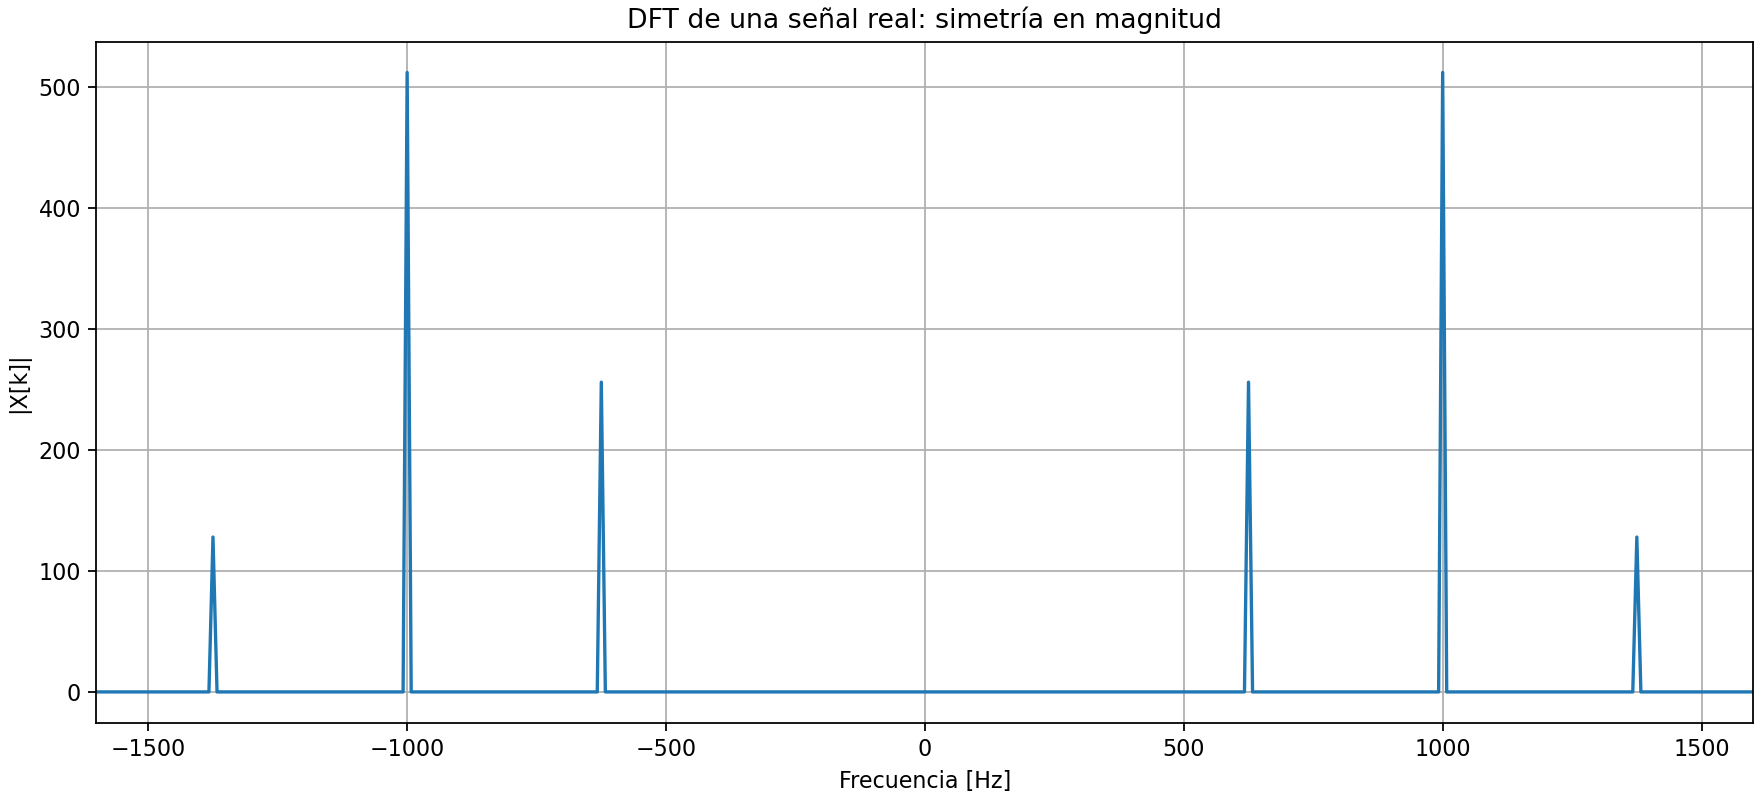
\includegraphics[width=.49\linewidth]{2_1d_simetria_conjugada.png}\hfill
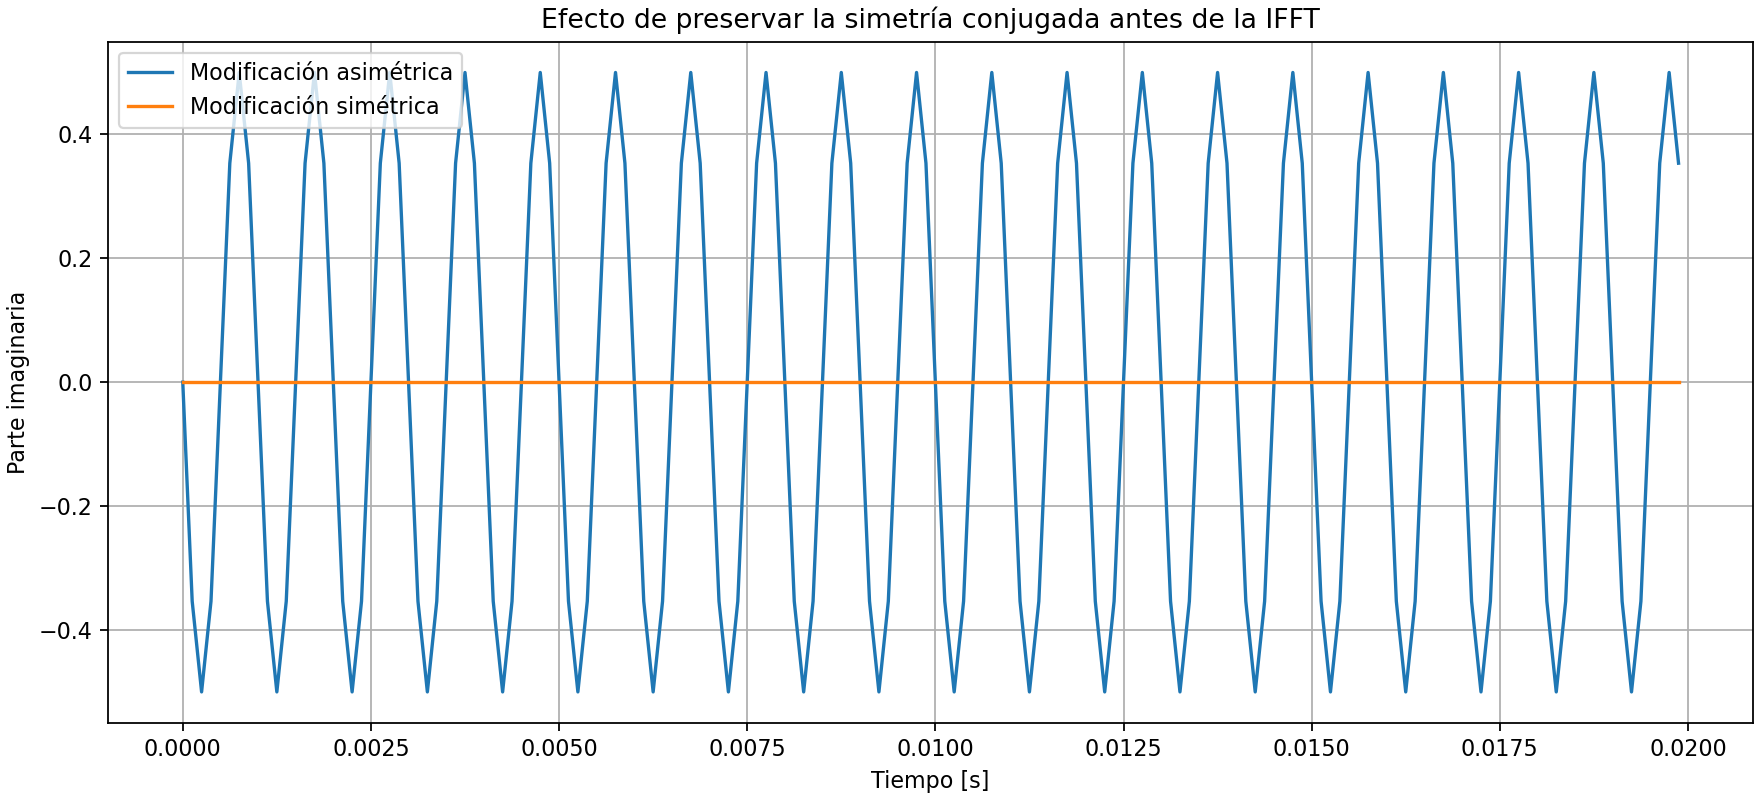
\includegraphics[width=.49\linewidth]{2_1d_ifft_simetria.png}
\caption{Simetría conjugada y efecto de modificar uno o ambos miembros del par.}\end{figure}
Anular solo $X[128]$ rompió la simetría y produjo una parte imaginaria de hasta 0.5. Al anular también $X[1024-128]$, cayó a $1.110\times10^{-16}$. El filtro debe conservar los pares conjugados; en PC lo hace con \ruta{rfft/irfft} y ganancias reales.

\section{Generación y caracterización de señales (2.2)}
La referencia $s$ contiene tonos de 300, 700 y 1100 Hz, amplitudes relativas $1$, $0.55$ y $0.30$, y fases $0^\circ$, $35^\circ$ y $-50^\circ$. Se suavizan sus extremos durante 20 ms. Cada captura tiene $L=8192$ muestras a $f_s=8000$ Hz, dura 1.024 s y usa bloques $N=1024$. Referencia, ruido y mezcla se normalizan con el mismo factor.

La mezcla es $x=s+r$. Para obtener una SNR objetivo de $\gamma$ dB, se ajusta la amplitud del ruido generado $\widetilde r$ mediante
\begin{equation}
r=\widetilde r\sqrt{\frac{\sum_n s^2[n]}{10^{\gamma/10}\sum_n\widetilde r^2[n]}}.
\end{equation}
\begin{table}[H]\centering\caption{Configuración y SNR verificada sobre las 8192 muestras originales.}
\begin{tabular}{clrrr}\toprule Caso & Ruido & Semilla & Objetivo (dB) & Obtenida (dB)\\\midrule
1&Tonal, 2150 Hz&202601&0&0.000000\\
2&Blanco gaussiano&202602&5&5.000000\\
3&Banda 900--1300 Hz&202603&3&3.000000\\\bottomrule
\end{tabular}\end{table}
La SNR difiere del objetivo en menos de $3\times10^{-14}$ dB. Para evaluar se usan los \ruta{muestras_exactas.npz}, sin cuantización WAV. Se guardan también tres WAV por caso, semillas y configuración. Las figuras muestran tiempo, magnitud, fase y energía por bandas.
\begin{figure}[p]\centering
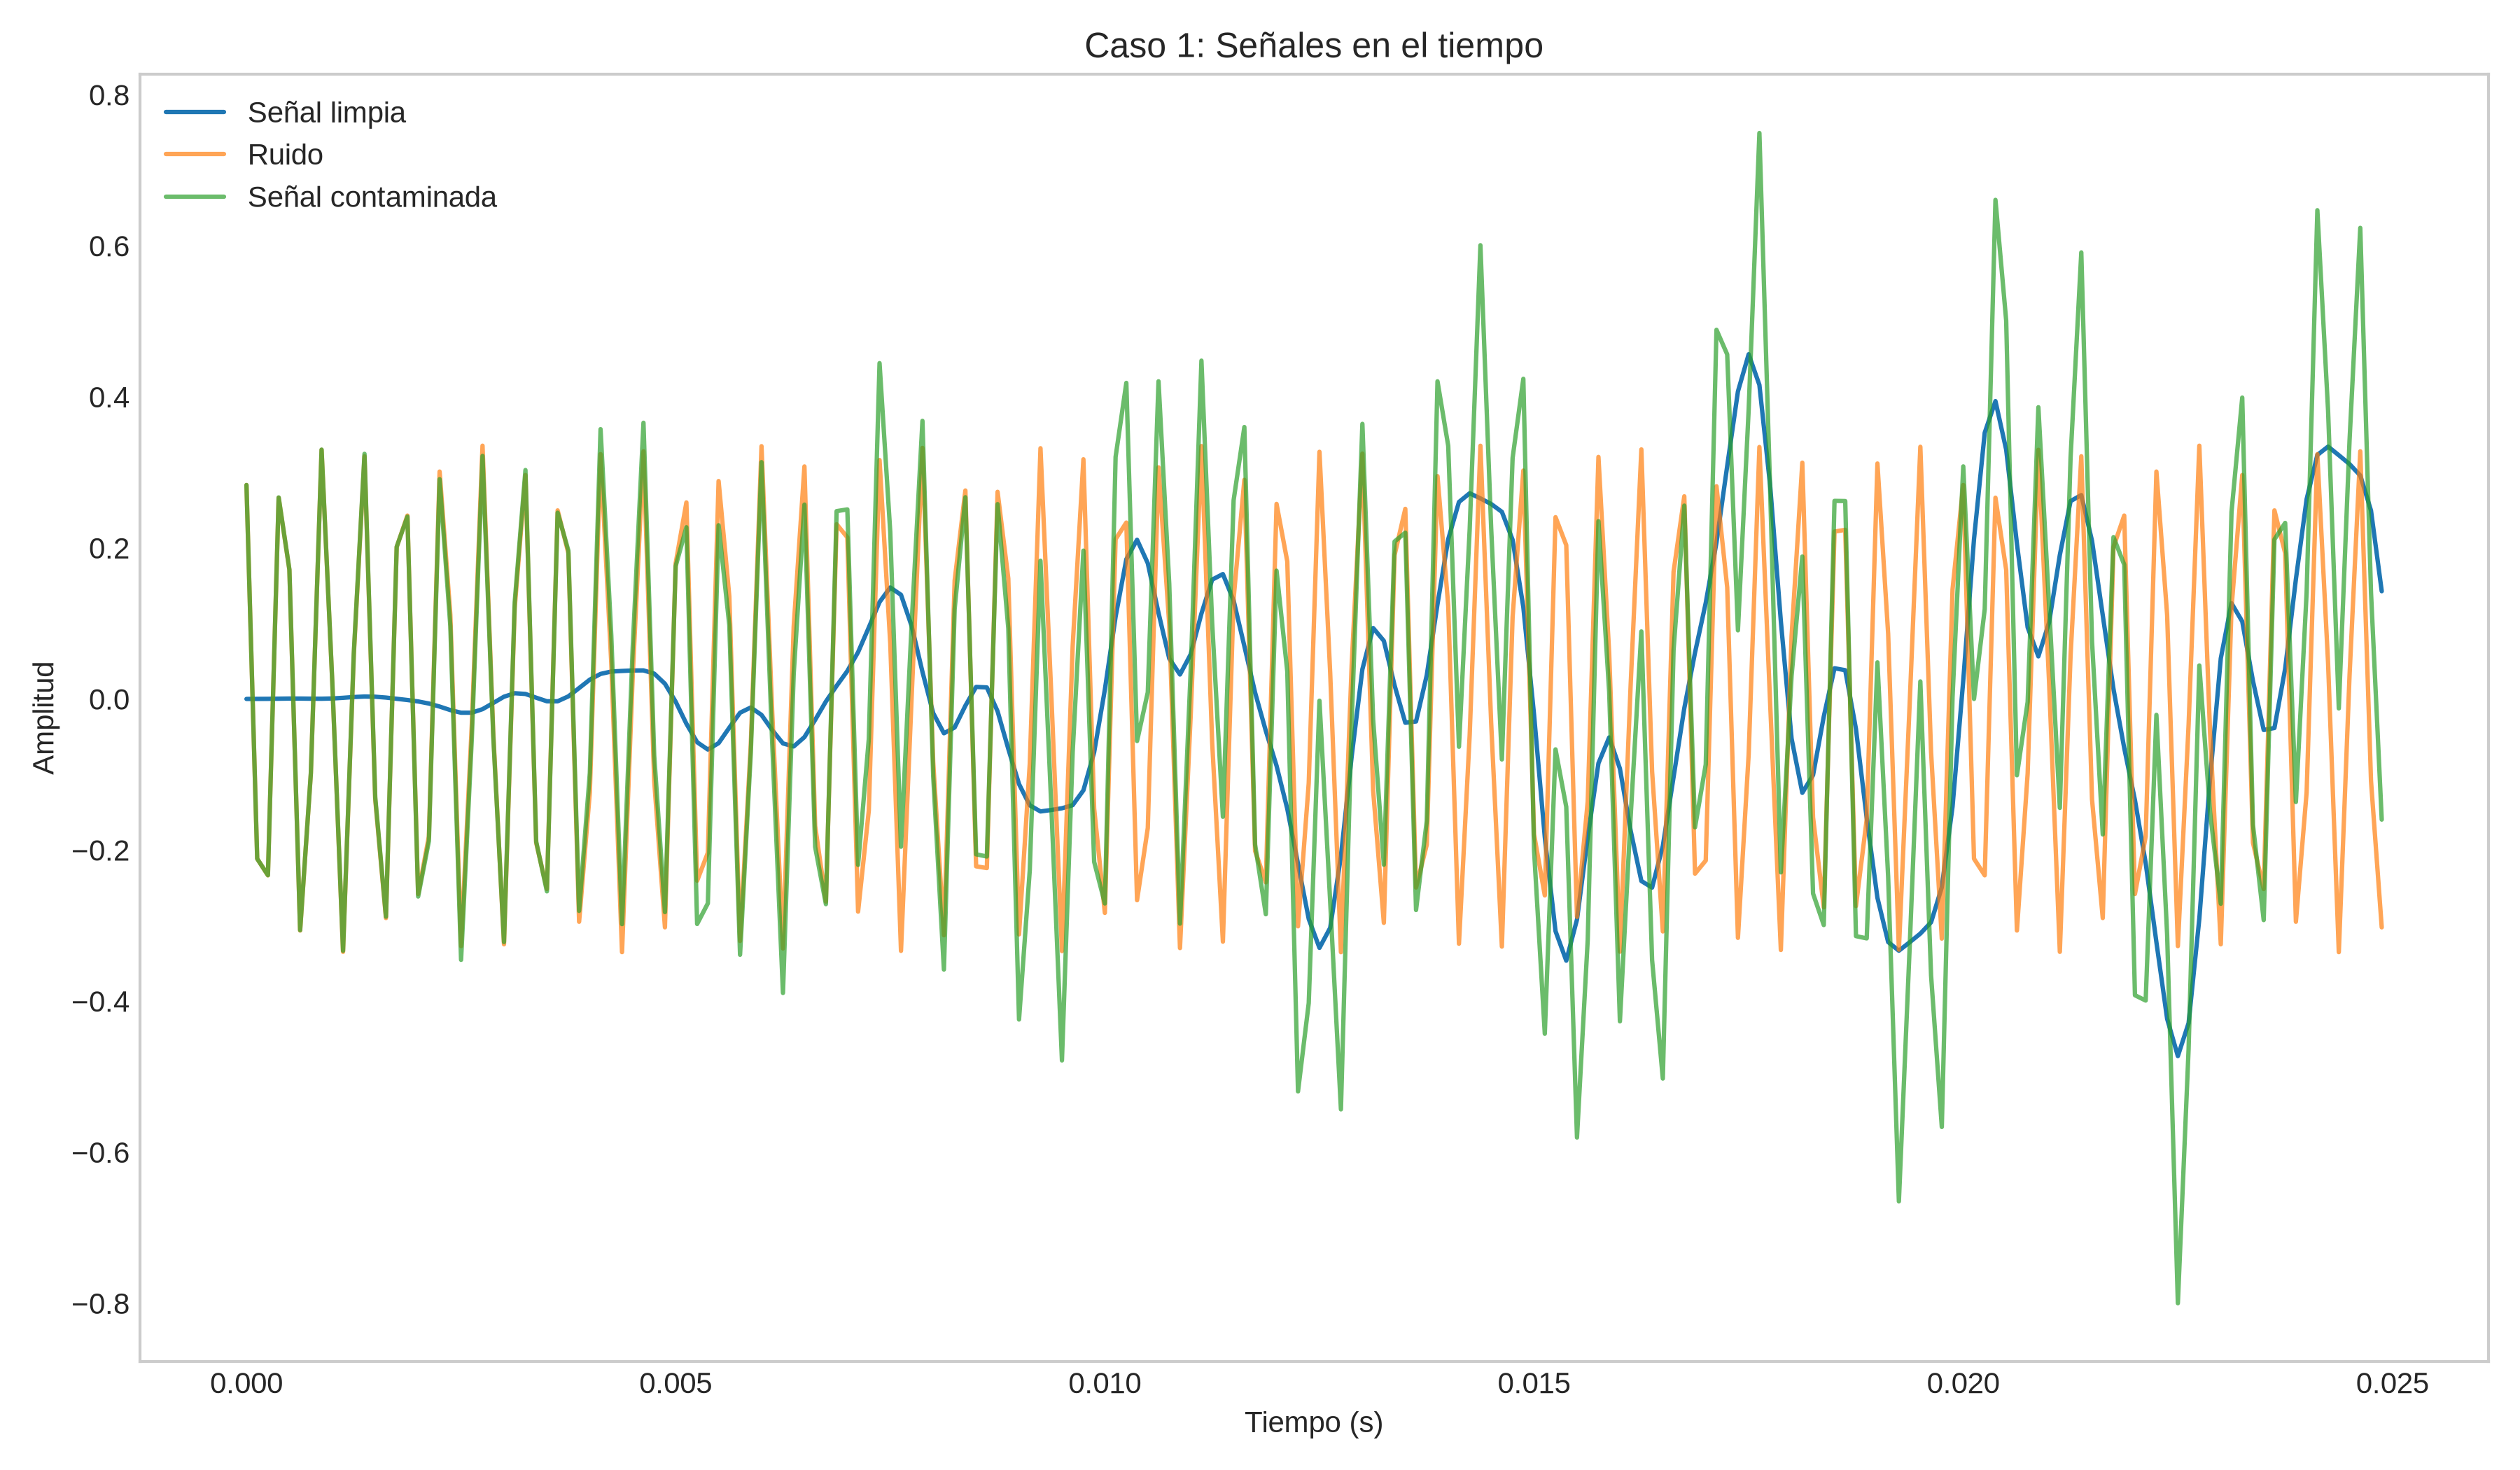
\includegraphics[width=.97\linewidth,height=.38\textheight,keepaspectratio]{generacion_1_temporal.png}\par
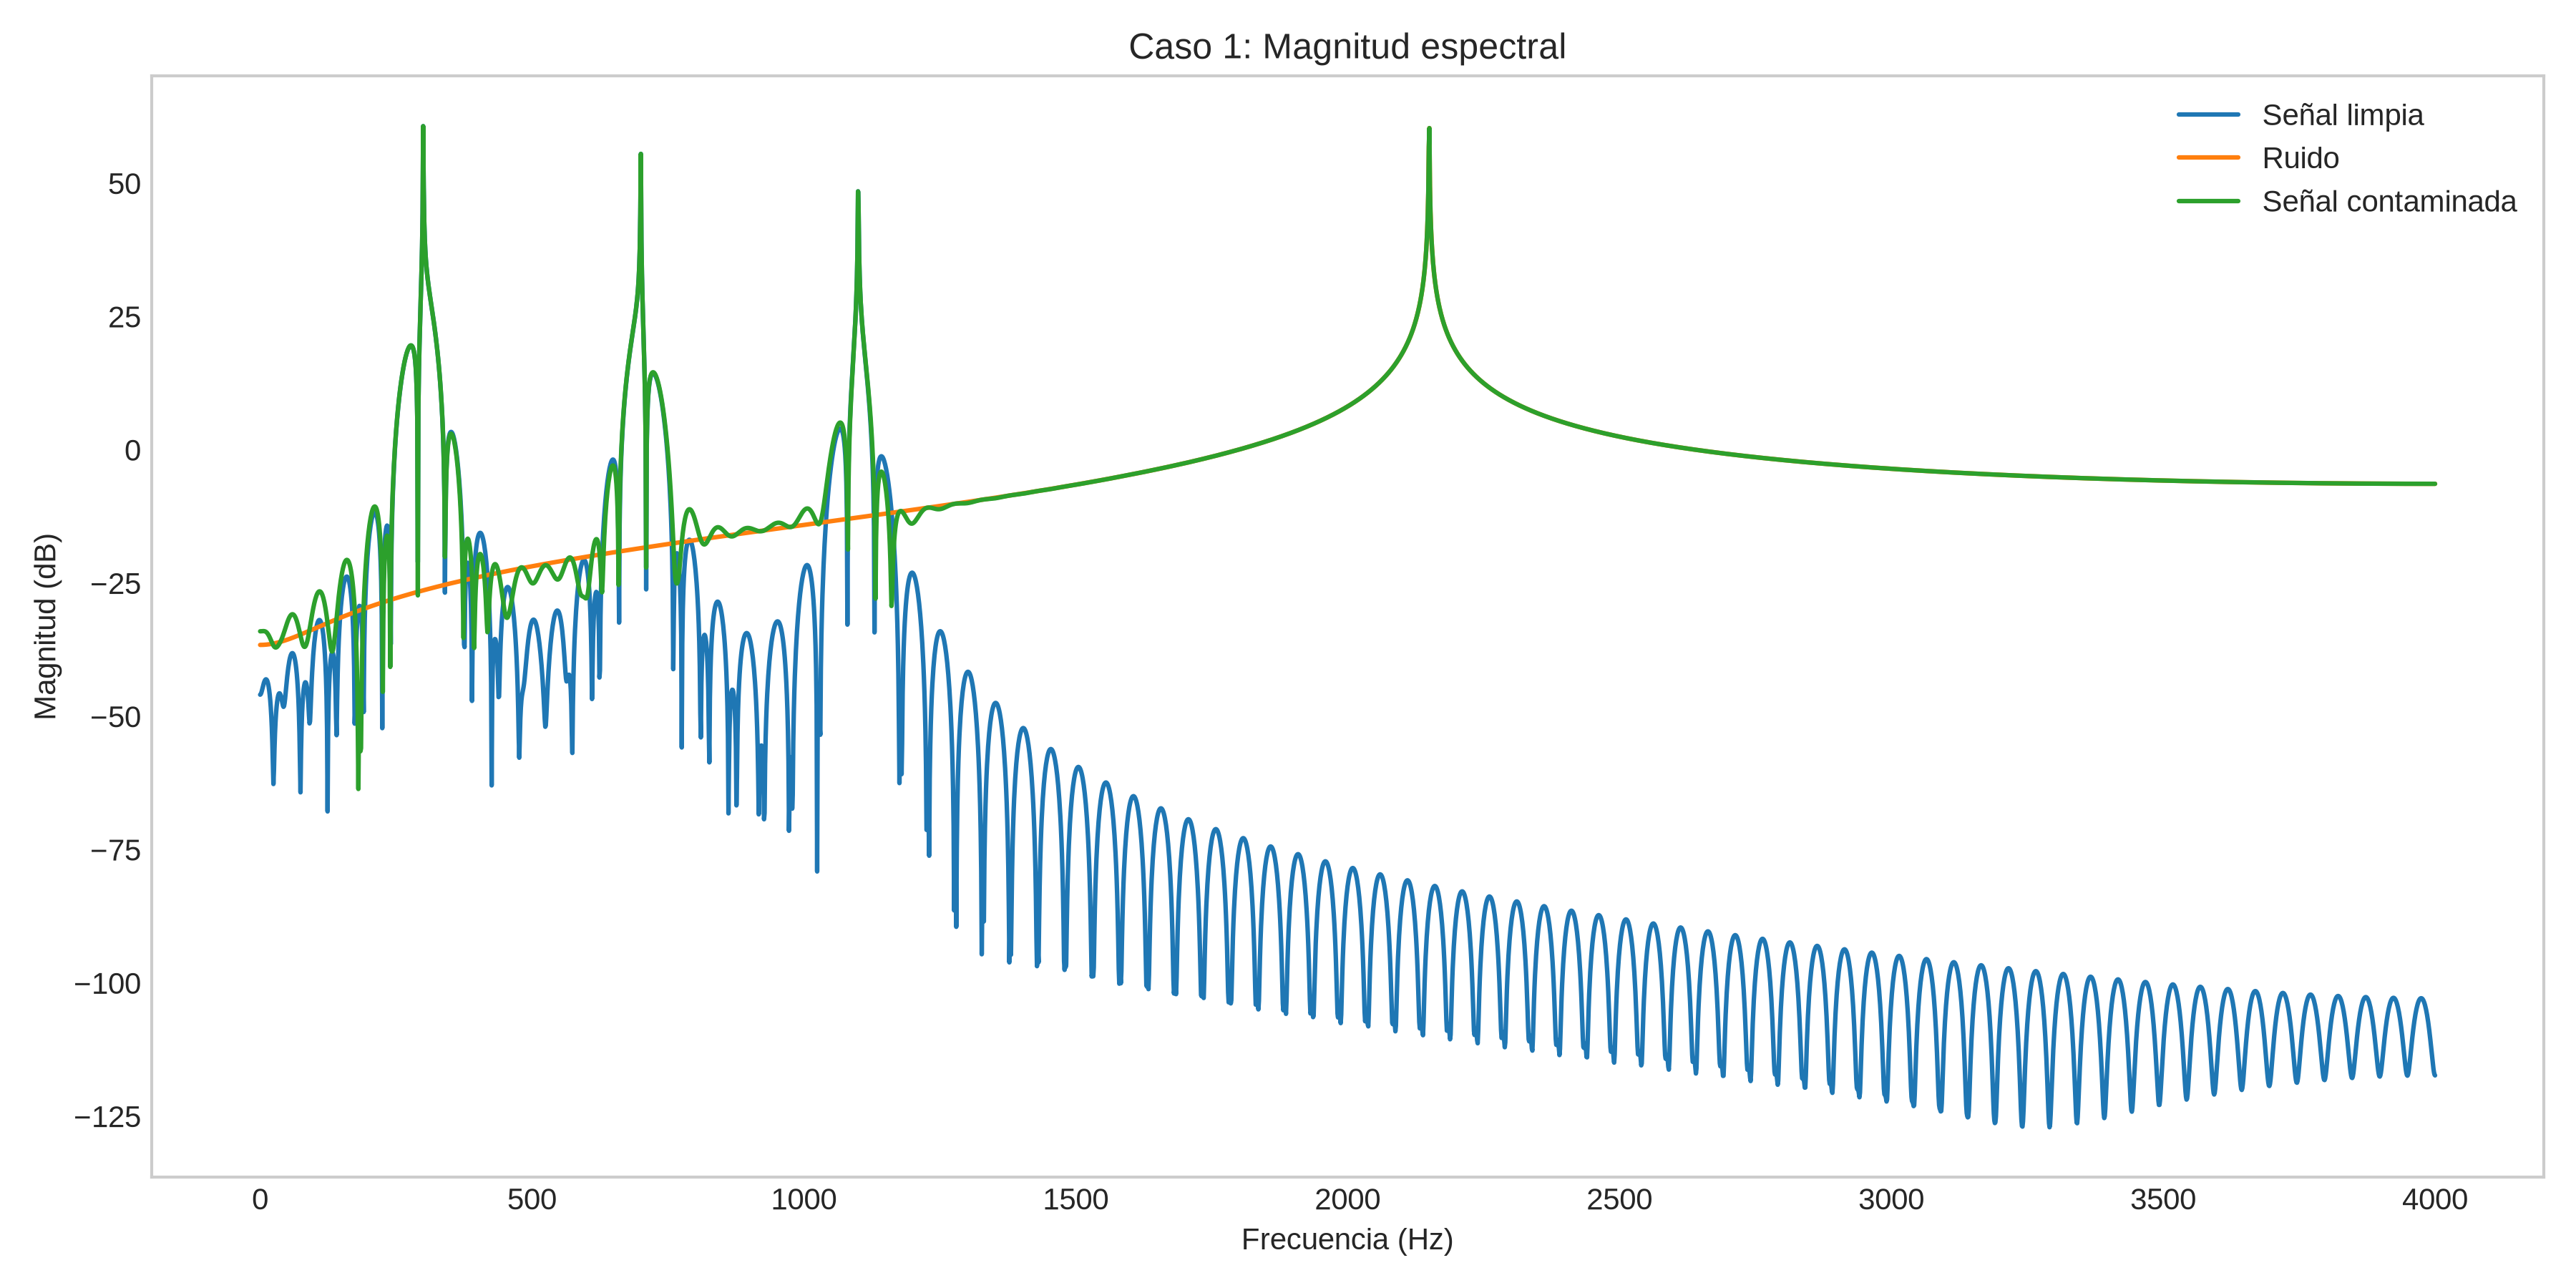
\includegraphics[width=.97\linewidth,height=.38\textheight,keepaspectratio]{generacion_1_magnitud.png}
\caption{Caso 1: Señales temporales y magnitud espectral. Resultados originales de 2.2.}\end{figure}
\begin{figure}[p]\centering
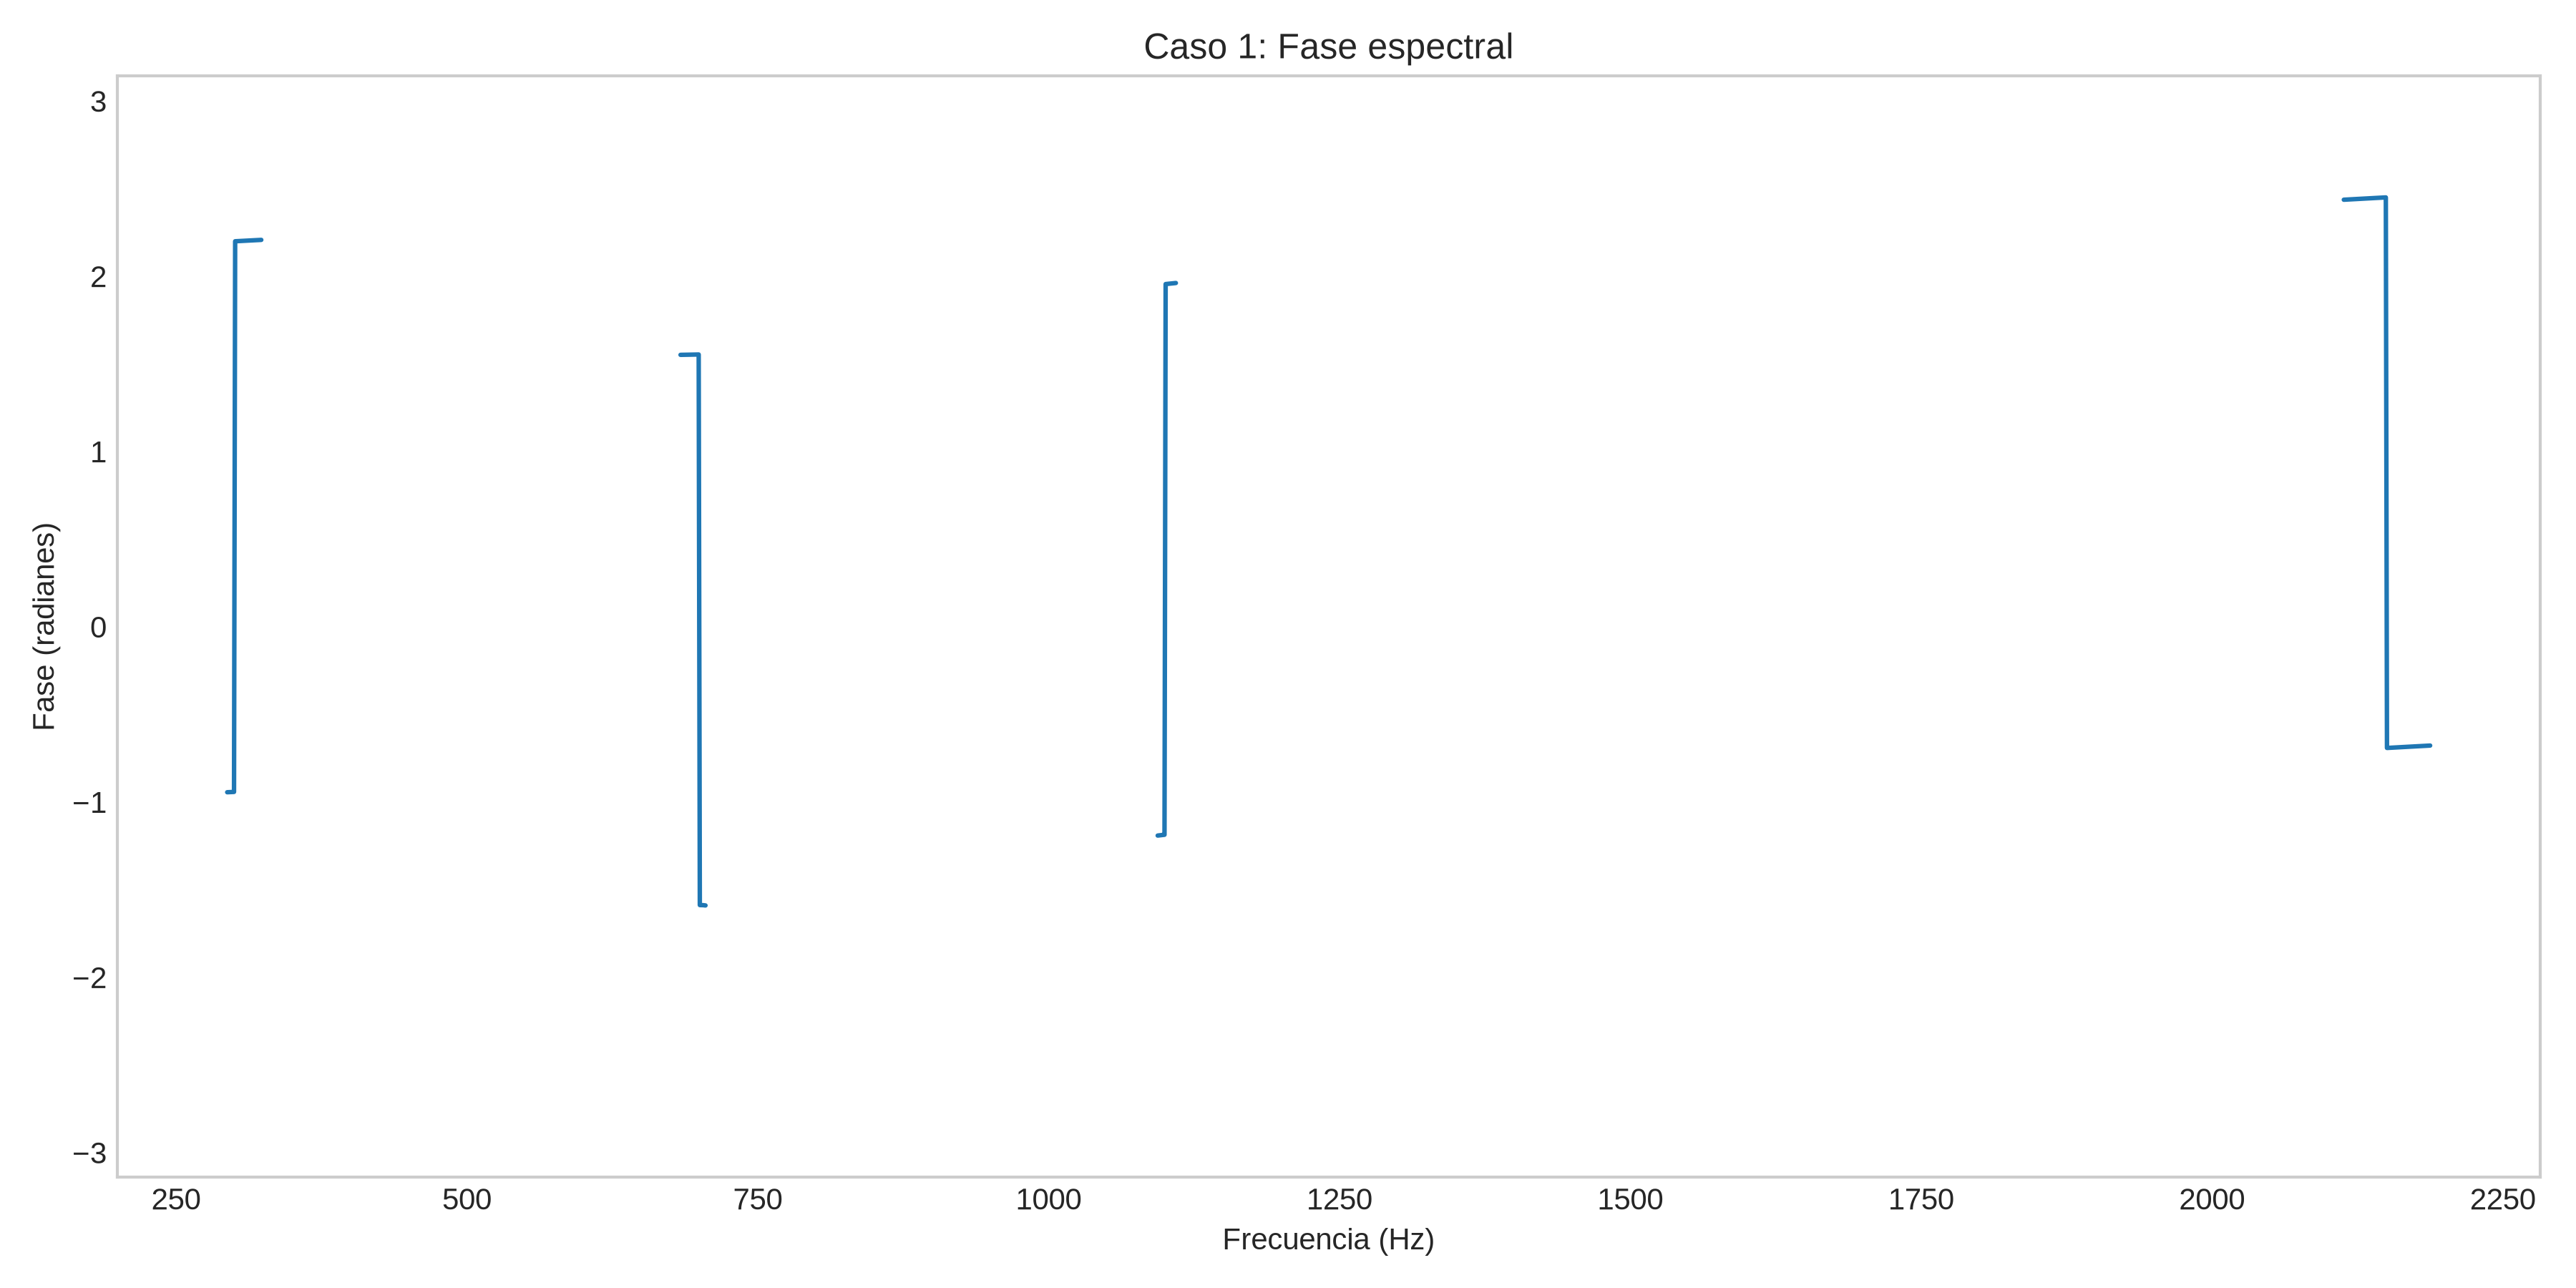
\includegraphics[width=.97\linewidth,height=.38\textheight,keepaspectratio]{generacion_1_fase.png}\par
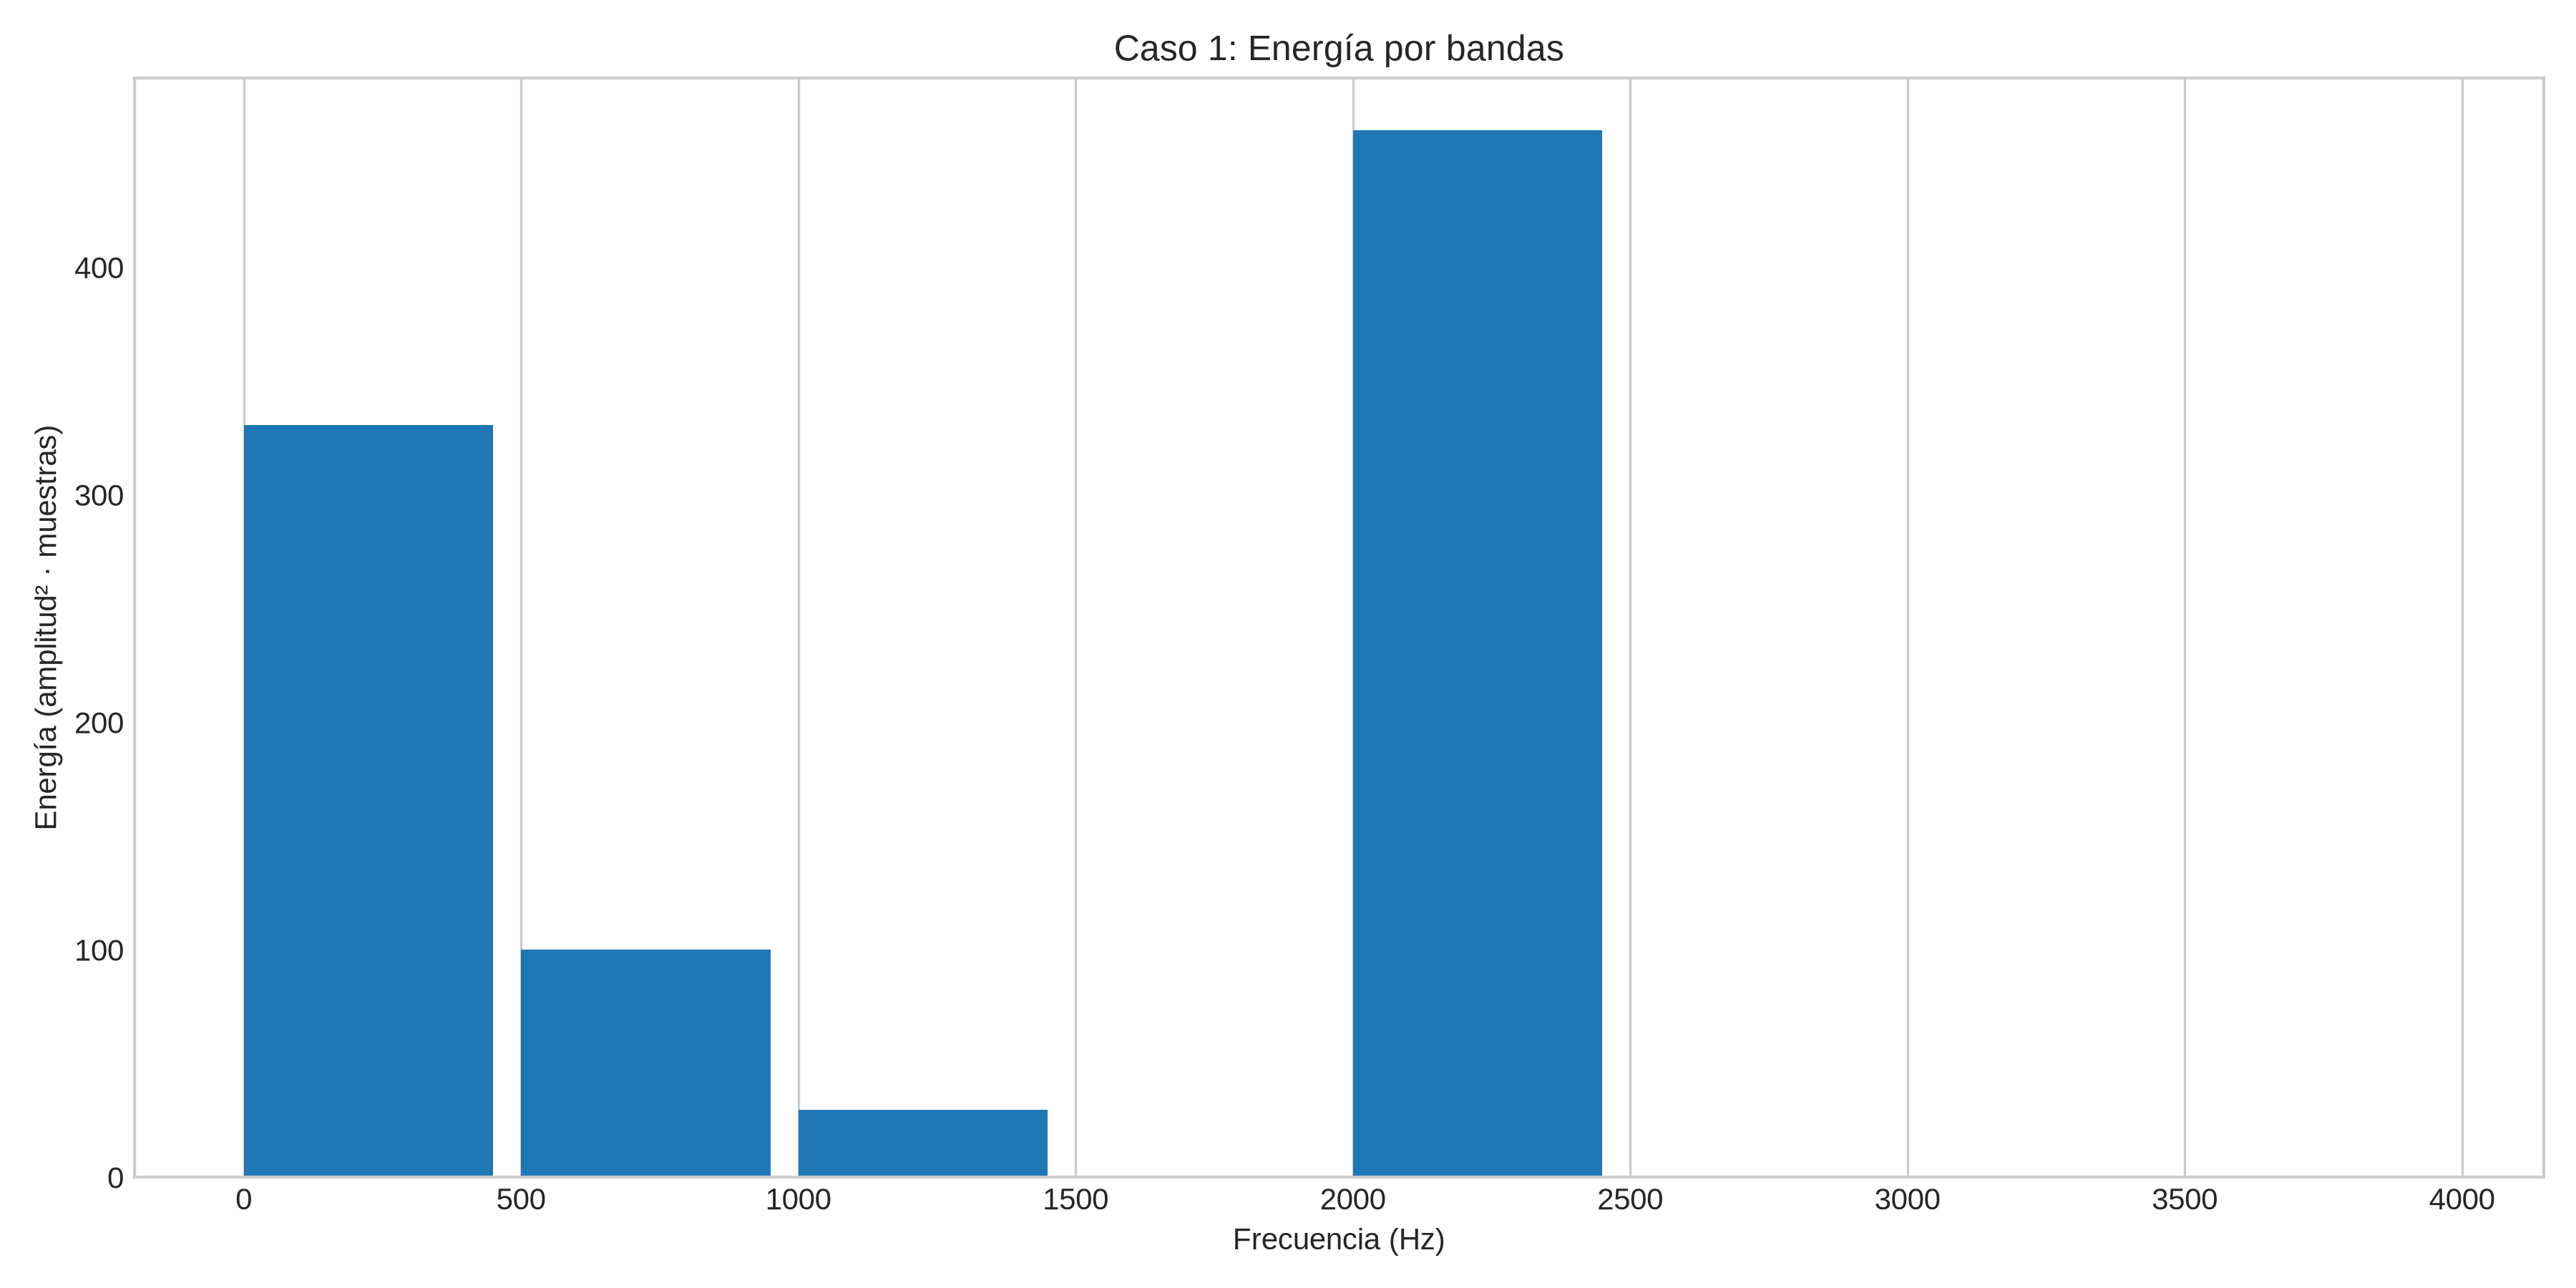
\includegraphics[width=.97\linewidth,height=.38\textheight,keepaspectratio]{generacion_1_energia.png}
\caption{Caso 1: Fase espectral y energía por bandas. Resultados originales de 2.2.}\end{figure}
\begin{figure}[p]\centering
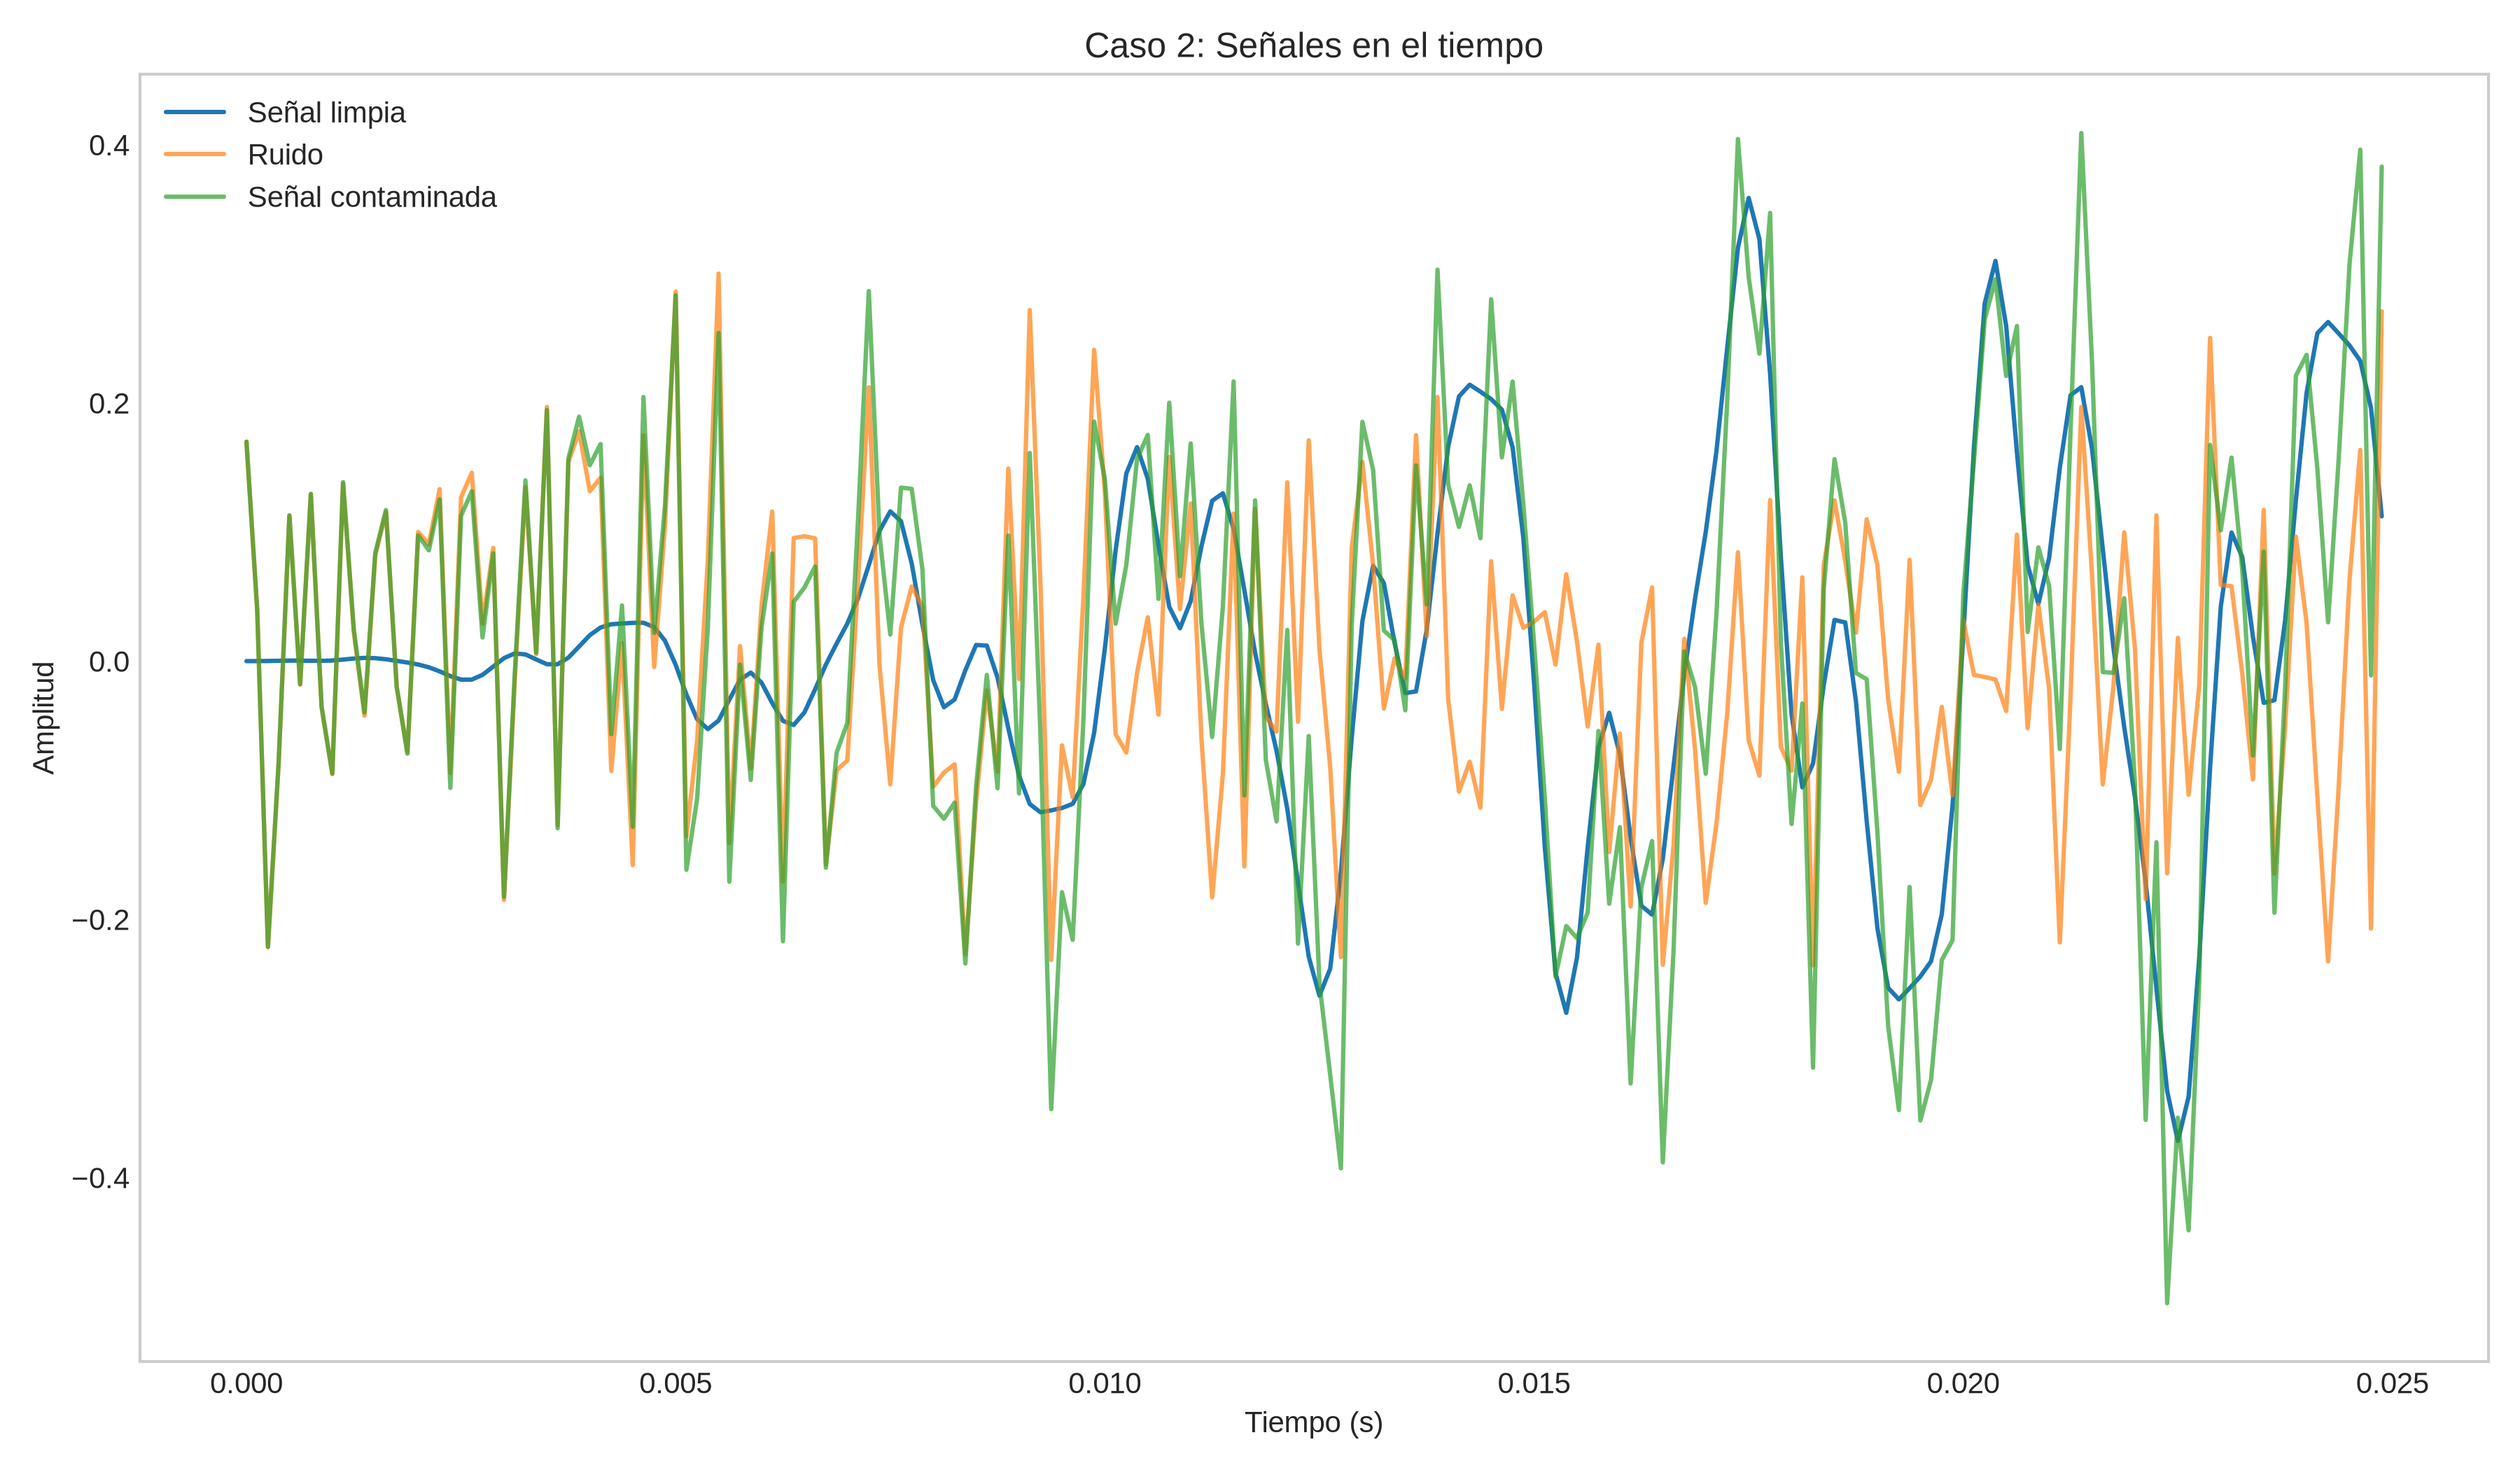
\includegraphics[width=.97\linewidth,height=.38\textheight,keepaspectratio]{generacion_2_temporal.png}\par
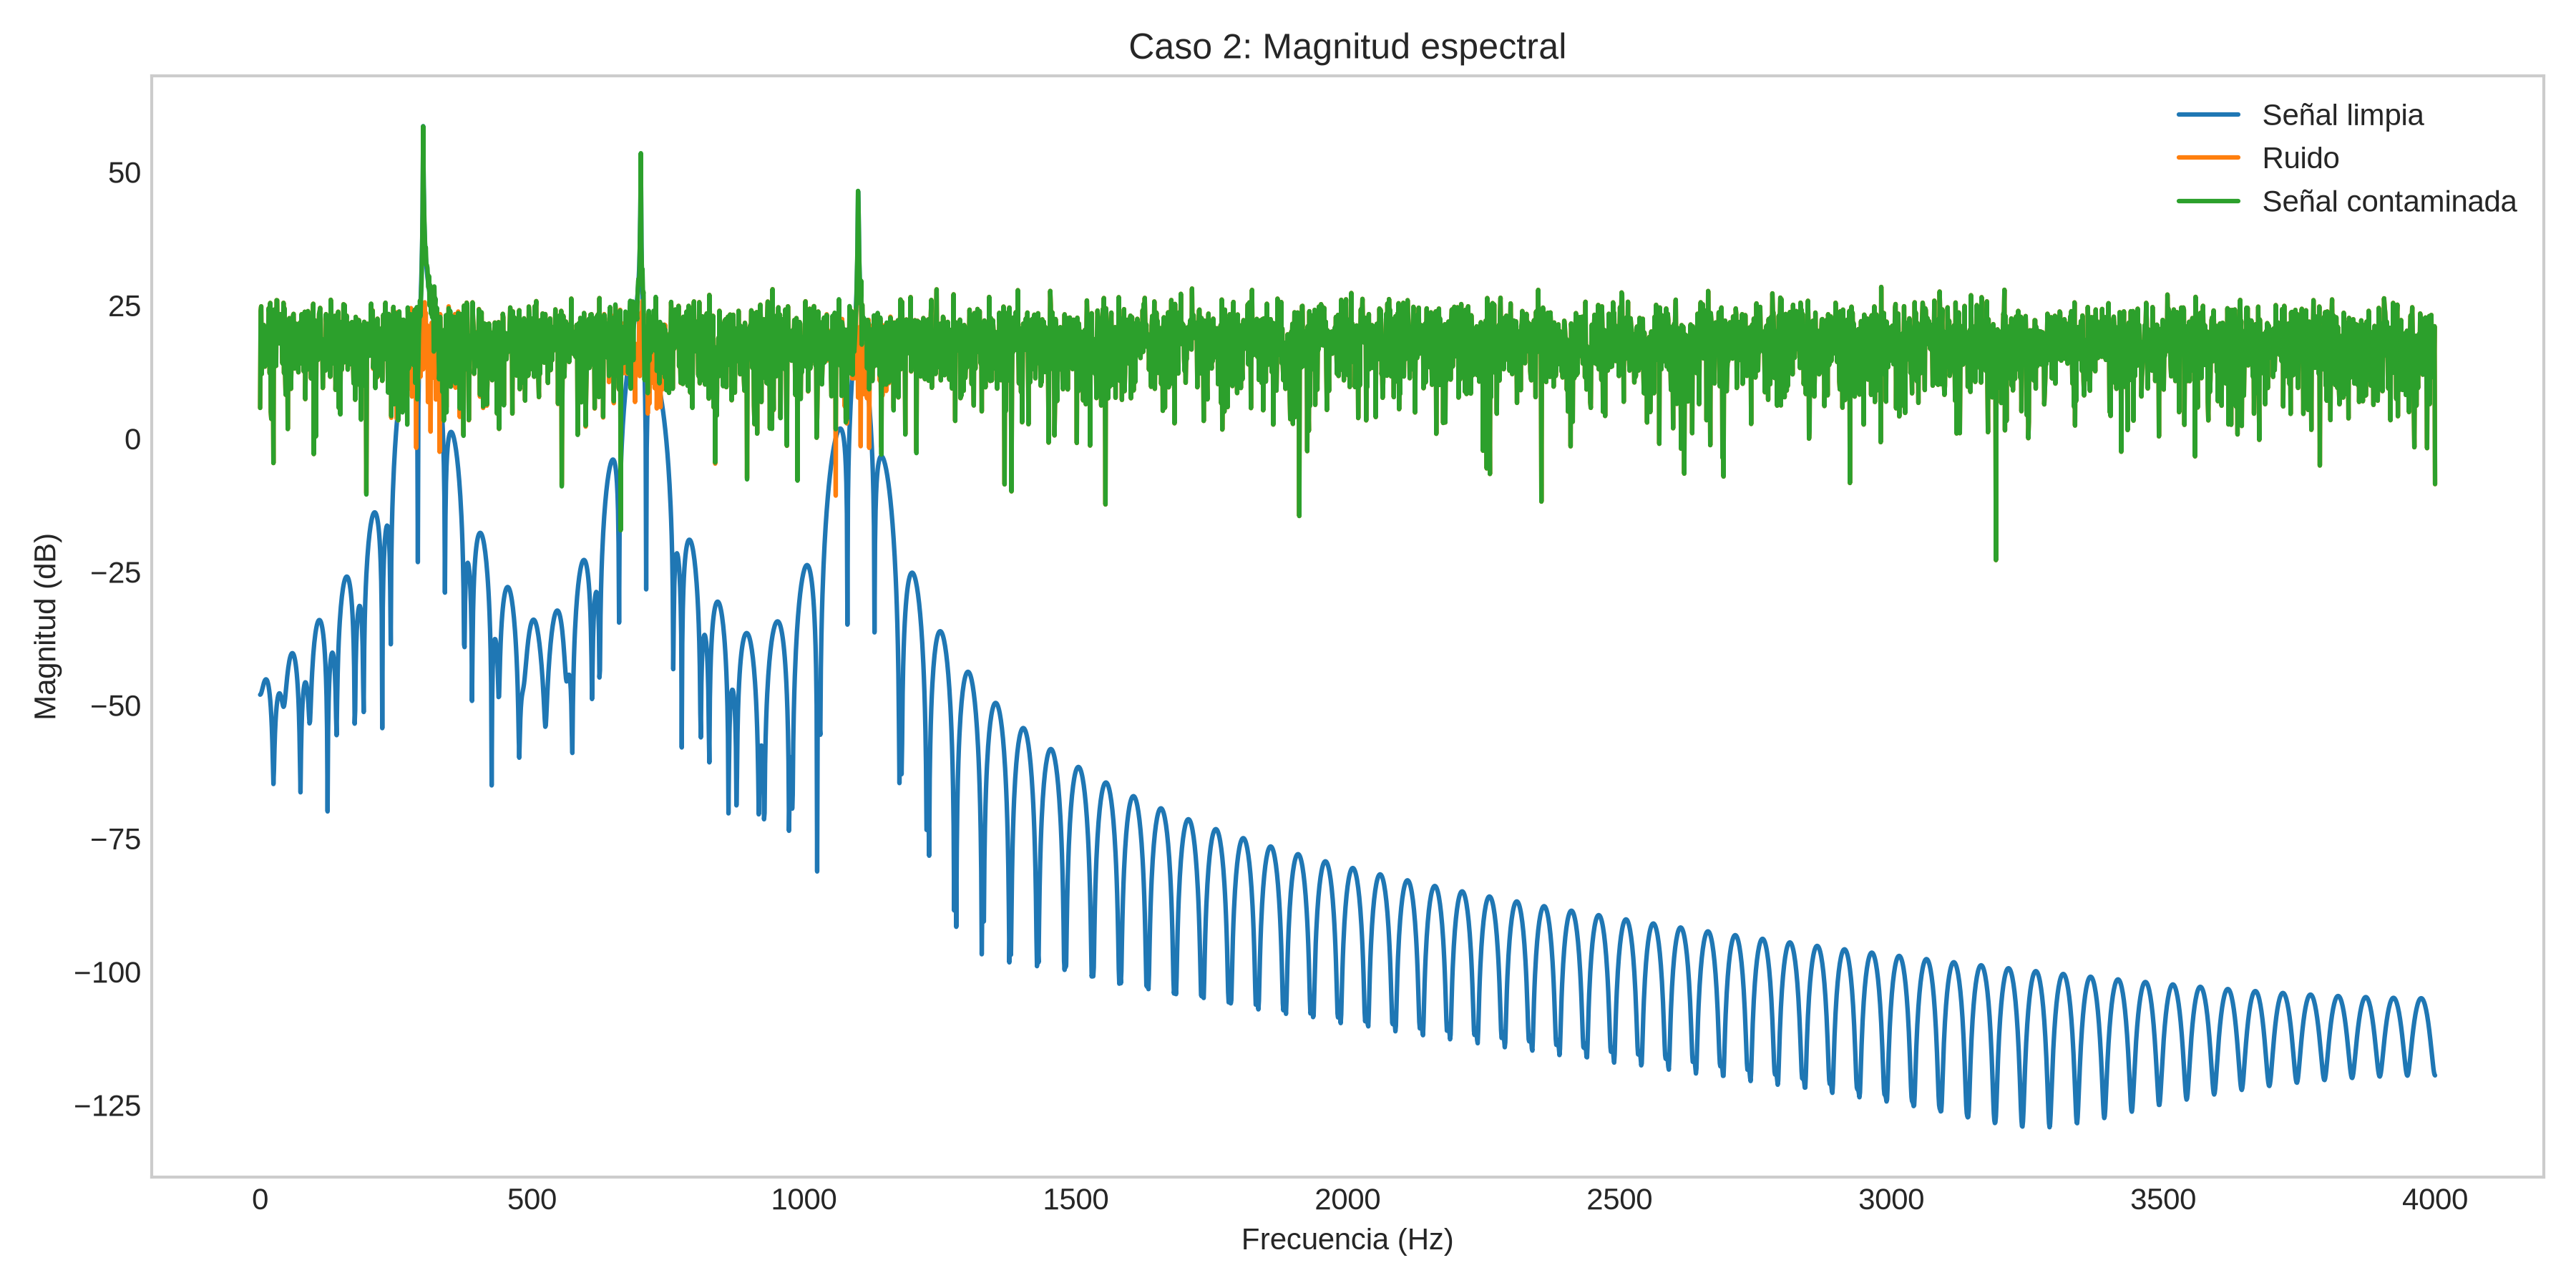
\includegraphics[width=.97\linewidth,height=.38\textheight,keepaspectratio]{generacion_2_magnitud.png}
\caption{Caso 2: Señales temporales y magnitud espectral. Resultados originales de 2.2.}\end{figure}
\begin{figure}[p]\centering
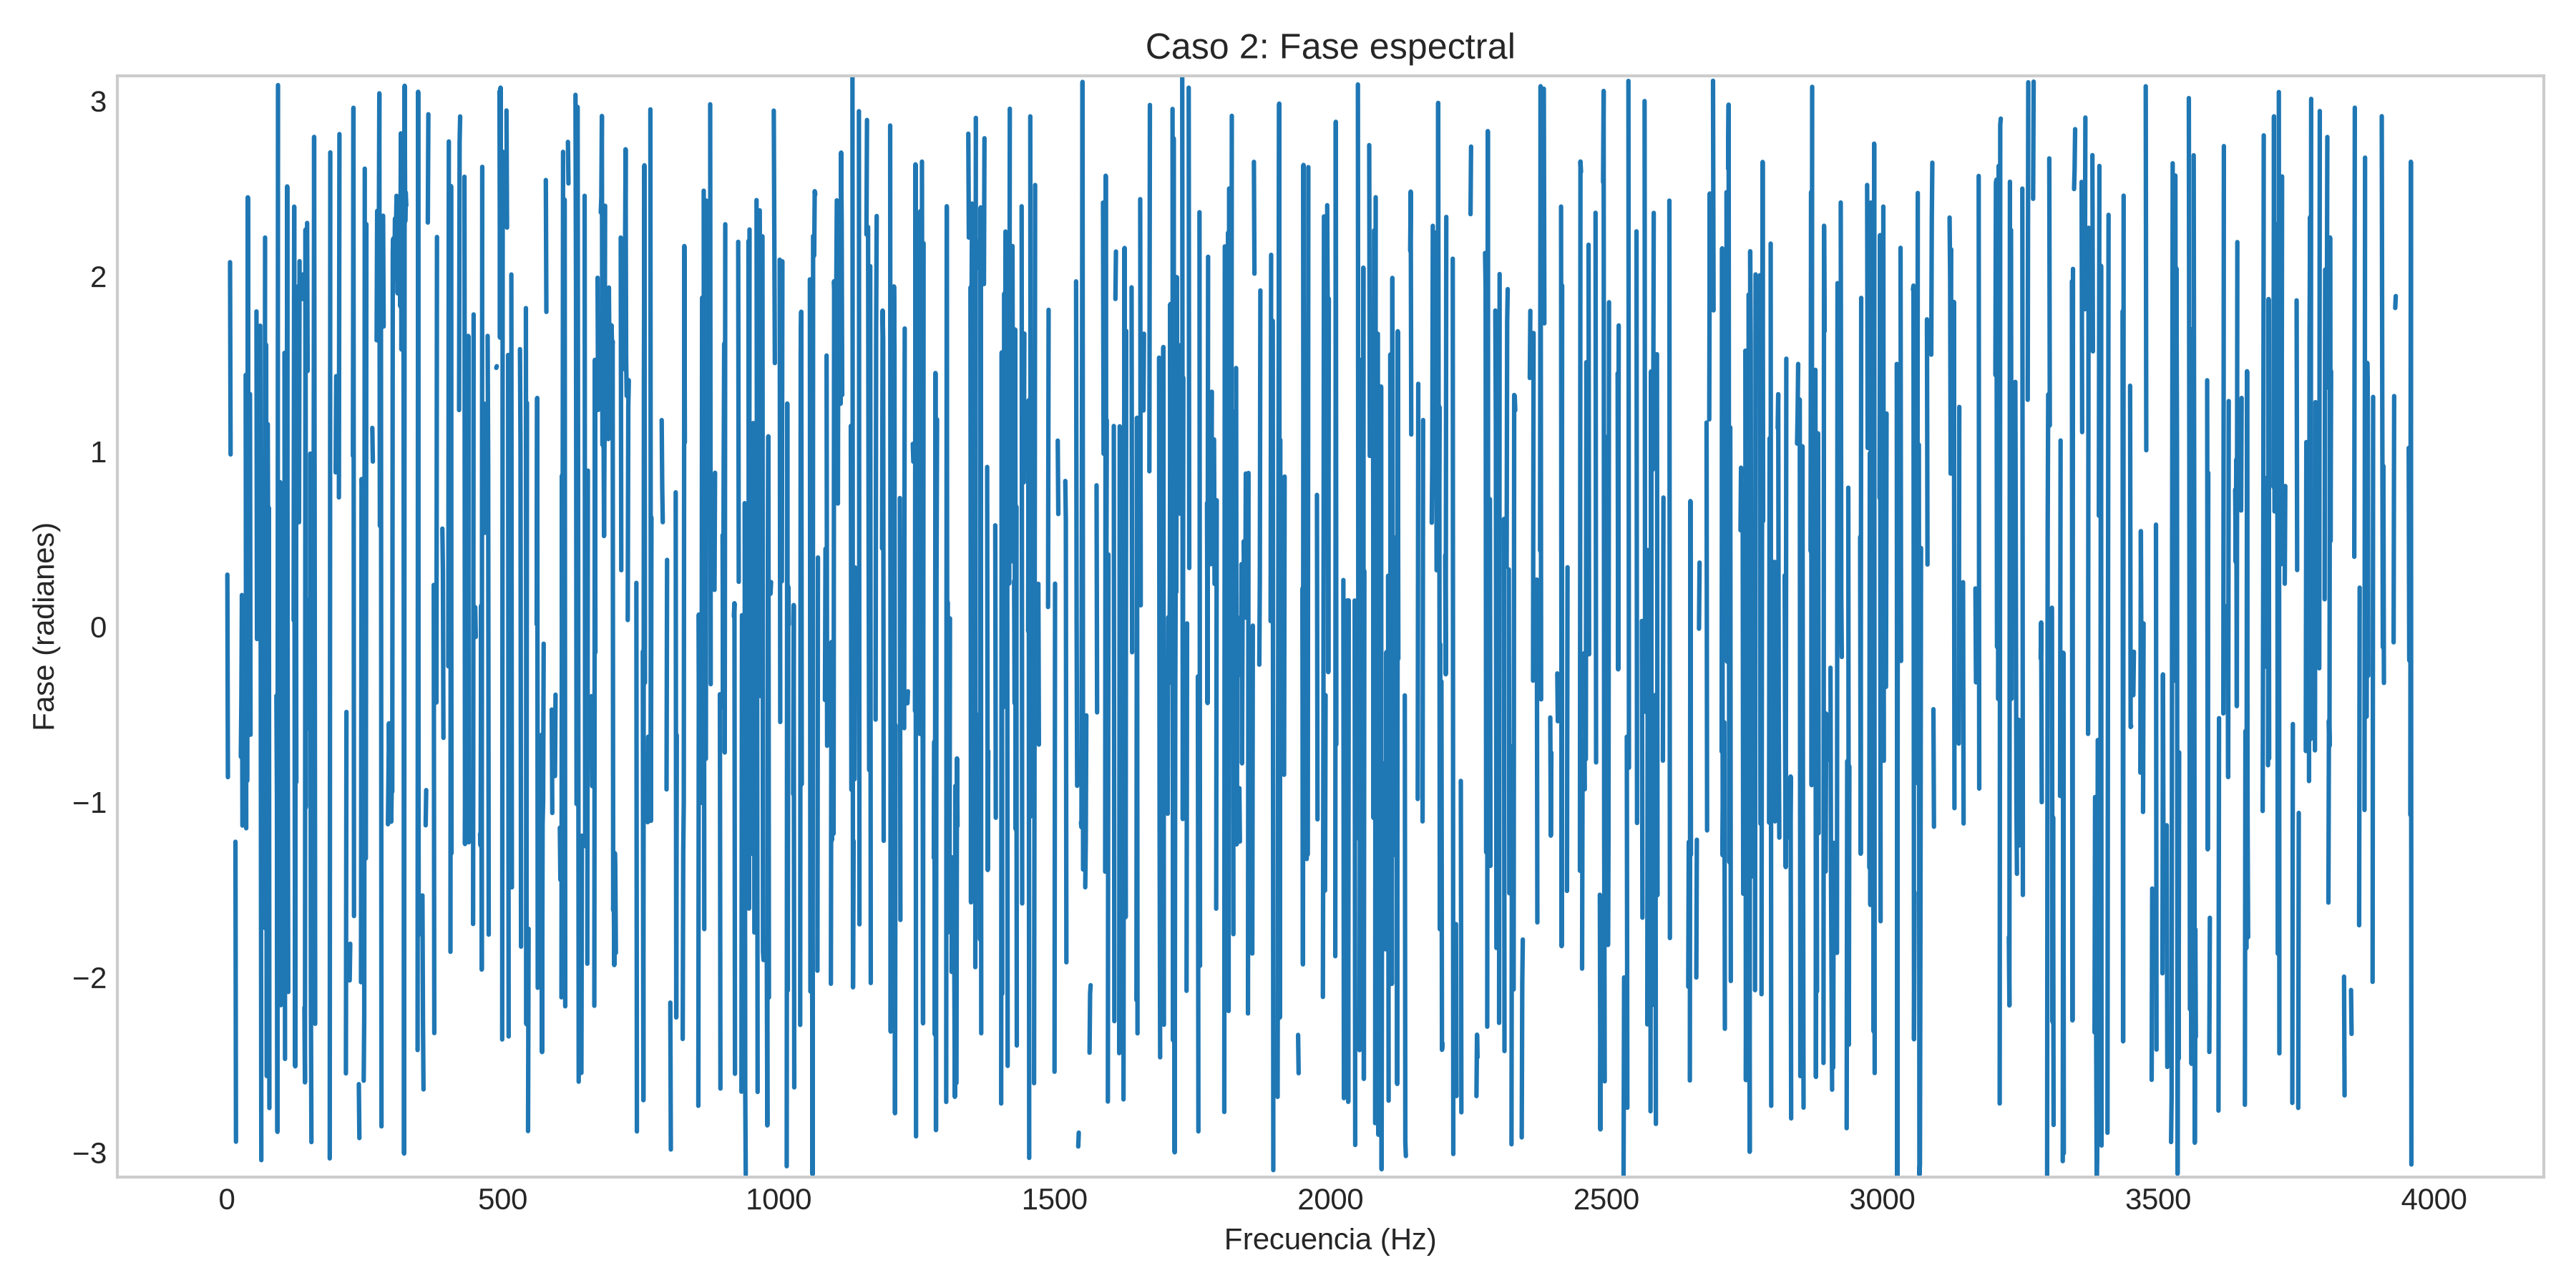
\includegraphics[width=.97\linewidth,height=.38\textheight,keepaspectratio]{generacion_2_fase.png}\par
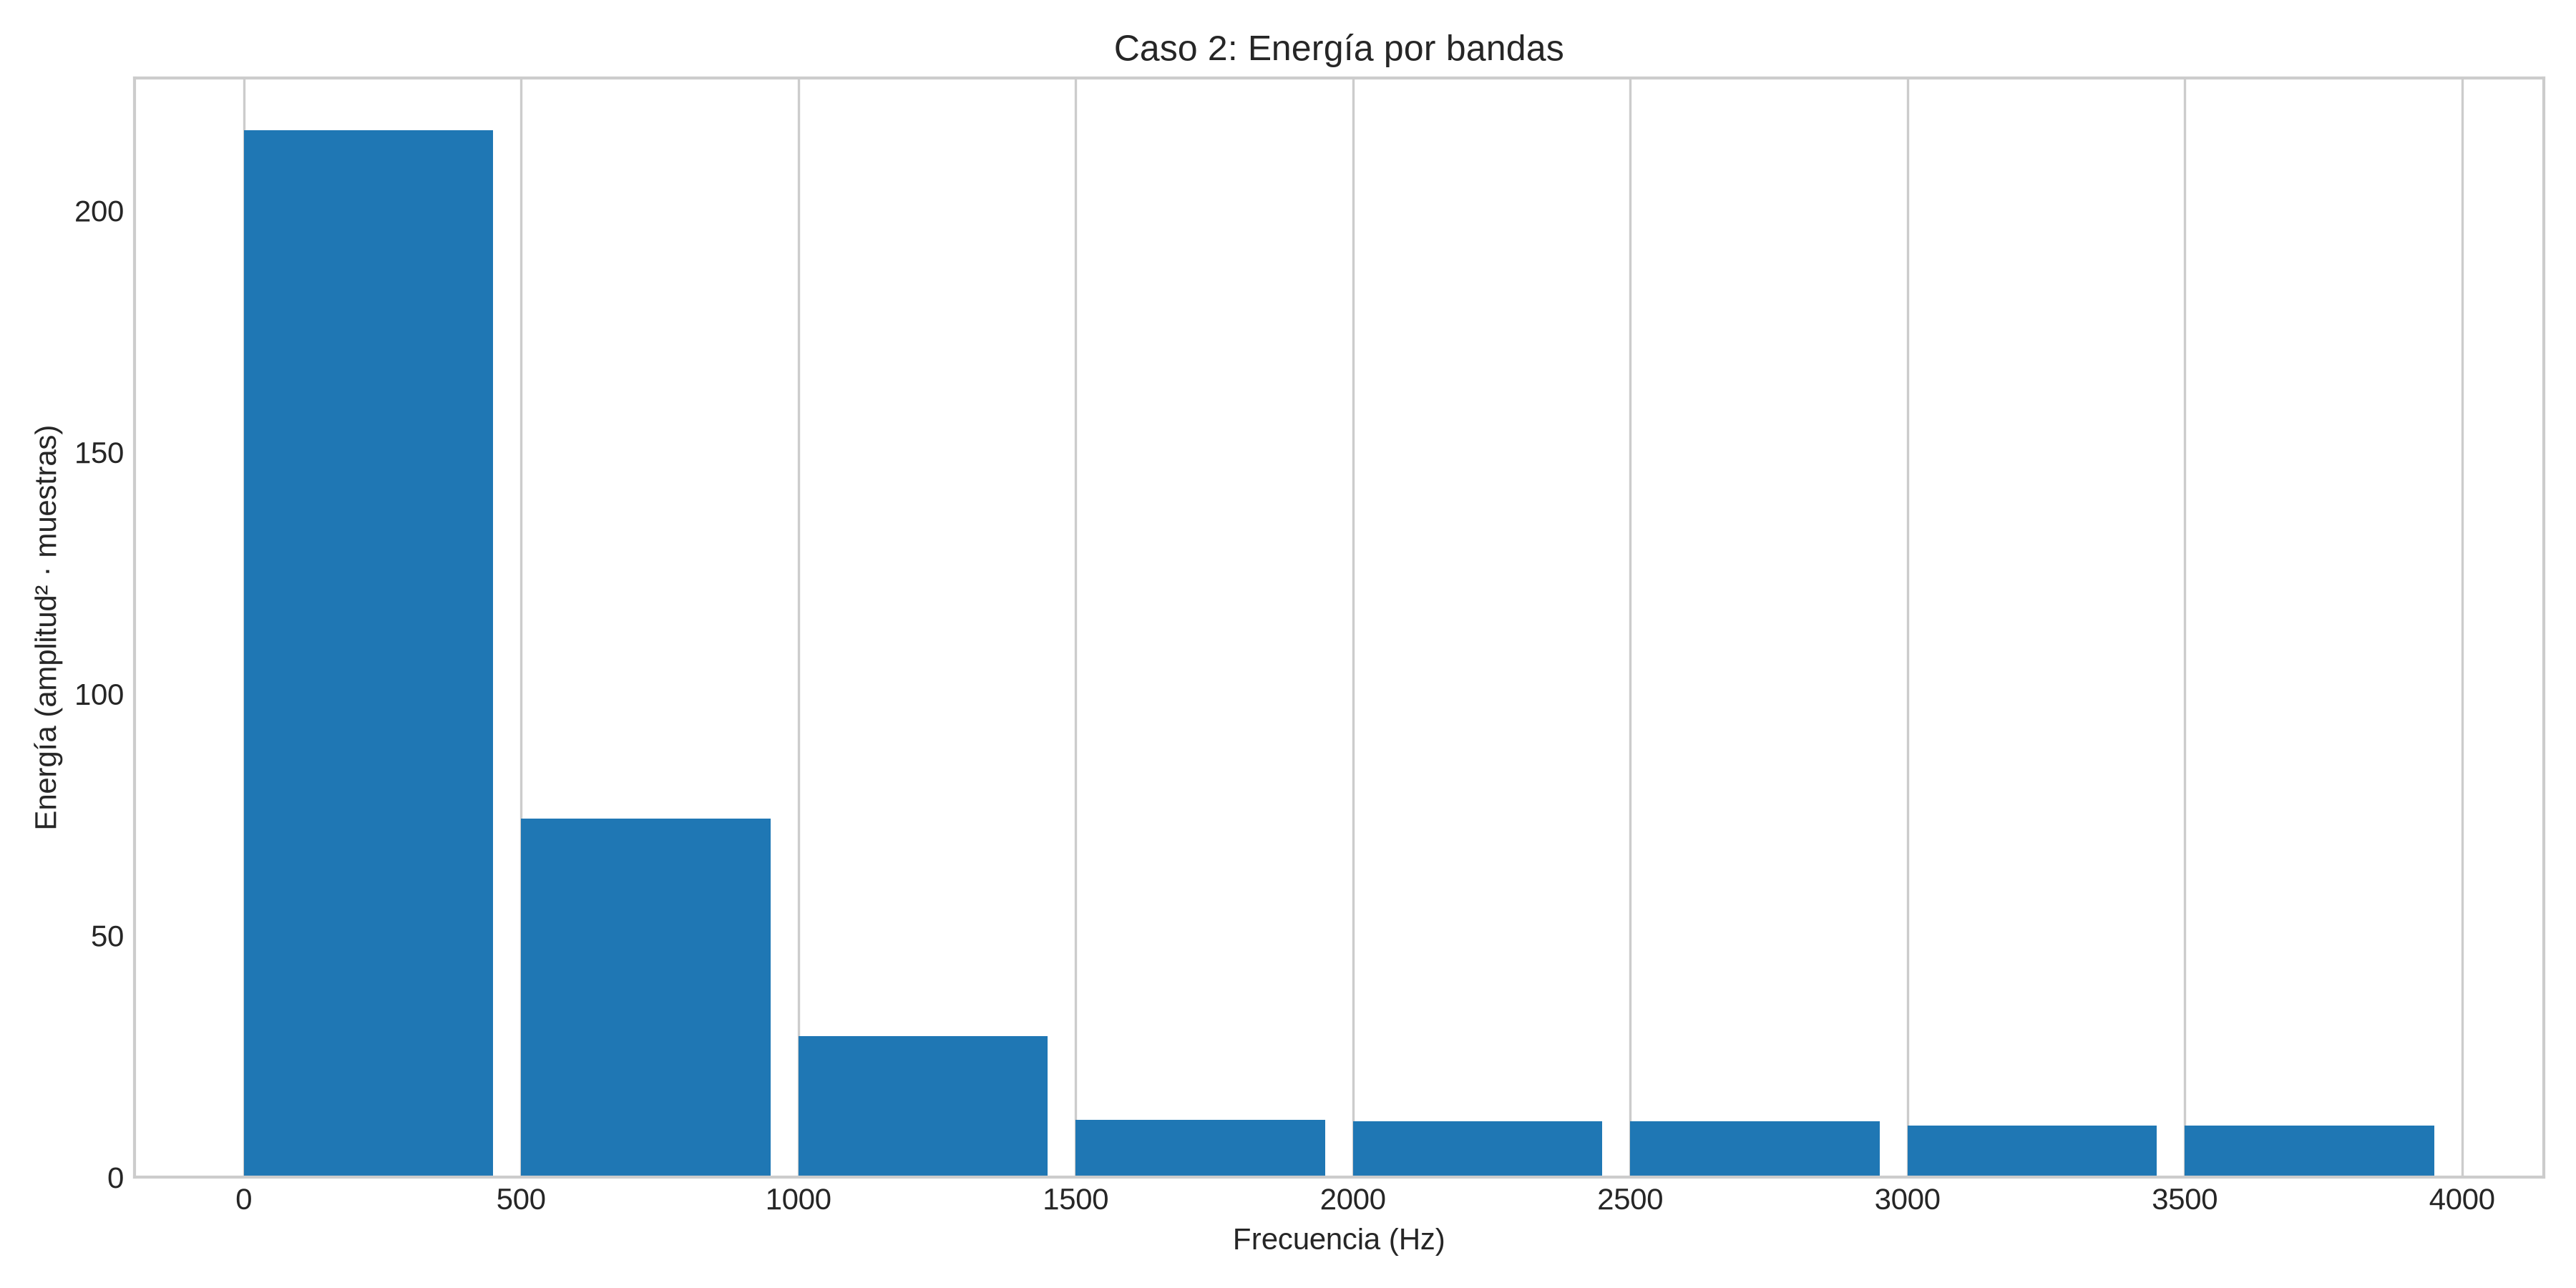
\includegraphics[width=.97\linewidth,height=.38\textheight,keepaspectratio]{generacion_2_energia.png}
\caption{Caso 2: Fase espectral y energía por bandas. Resultados originales de 2.2.}\end{figure}
\begin{figure}[p]\centering
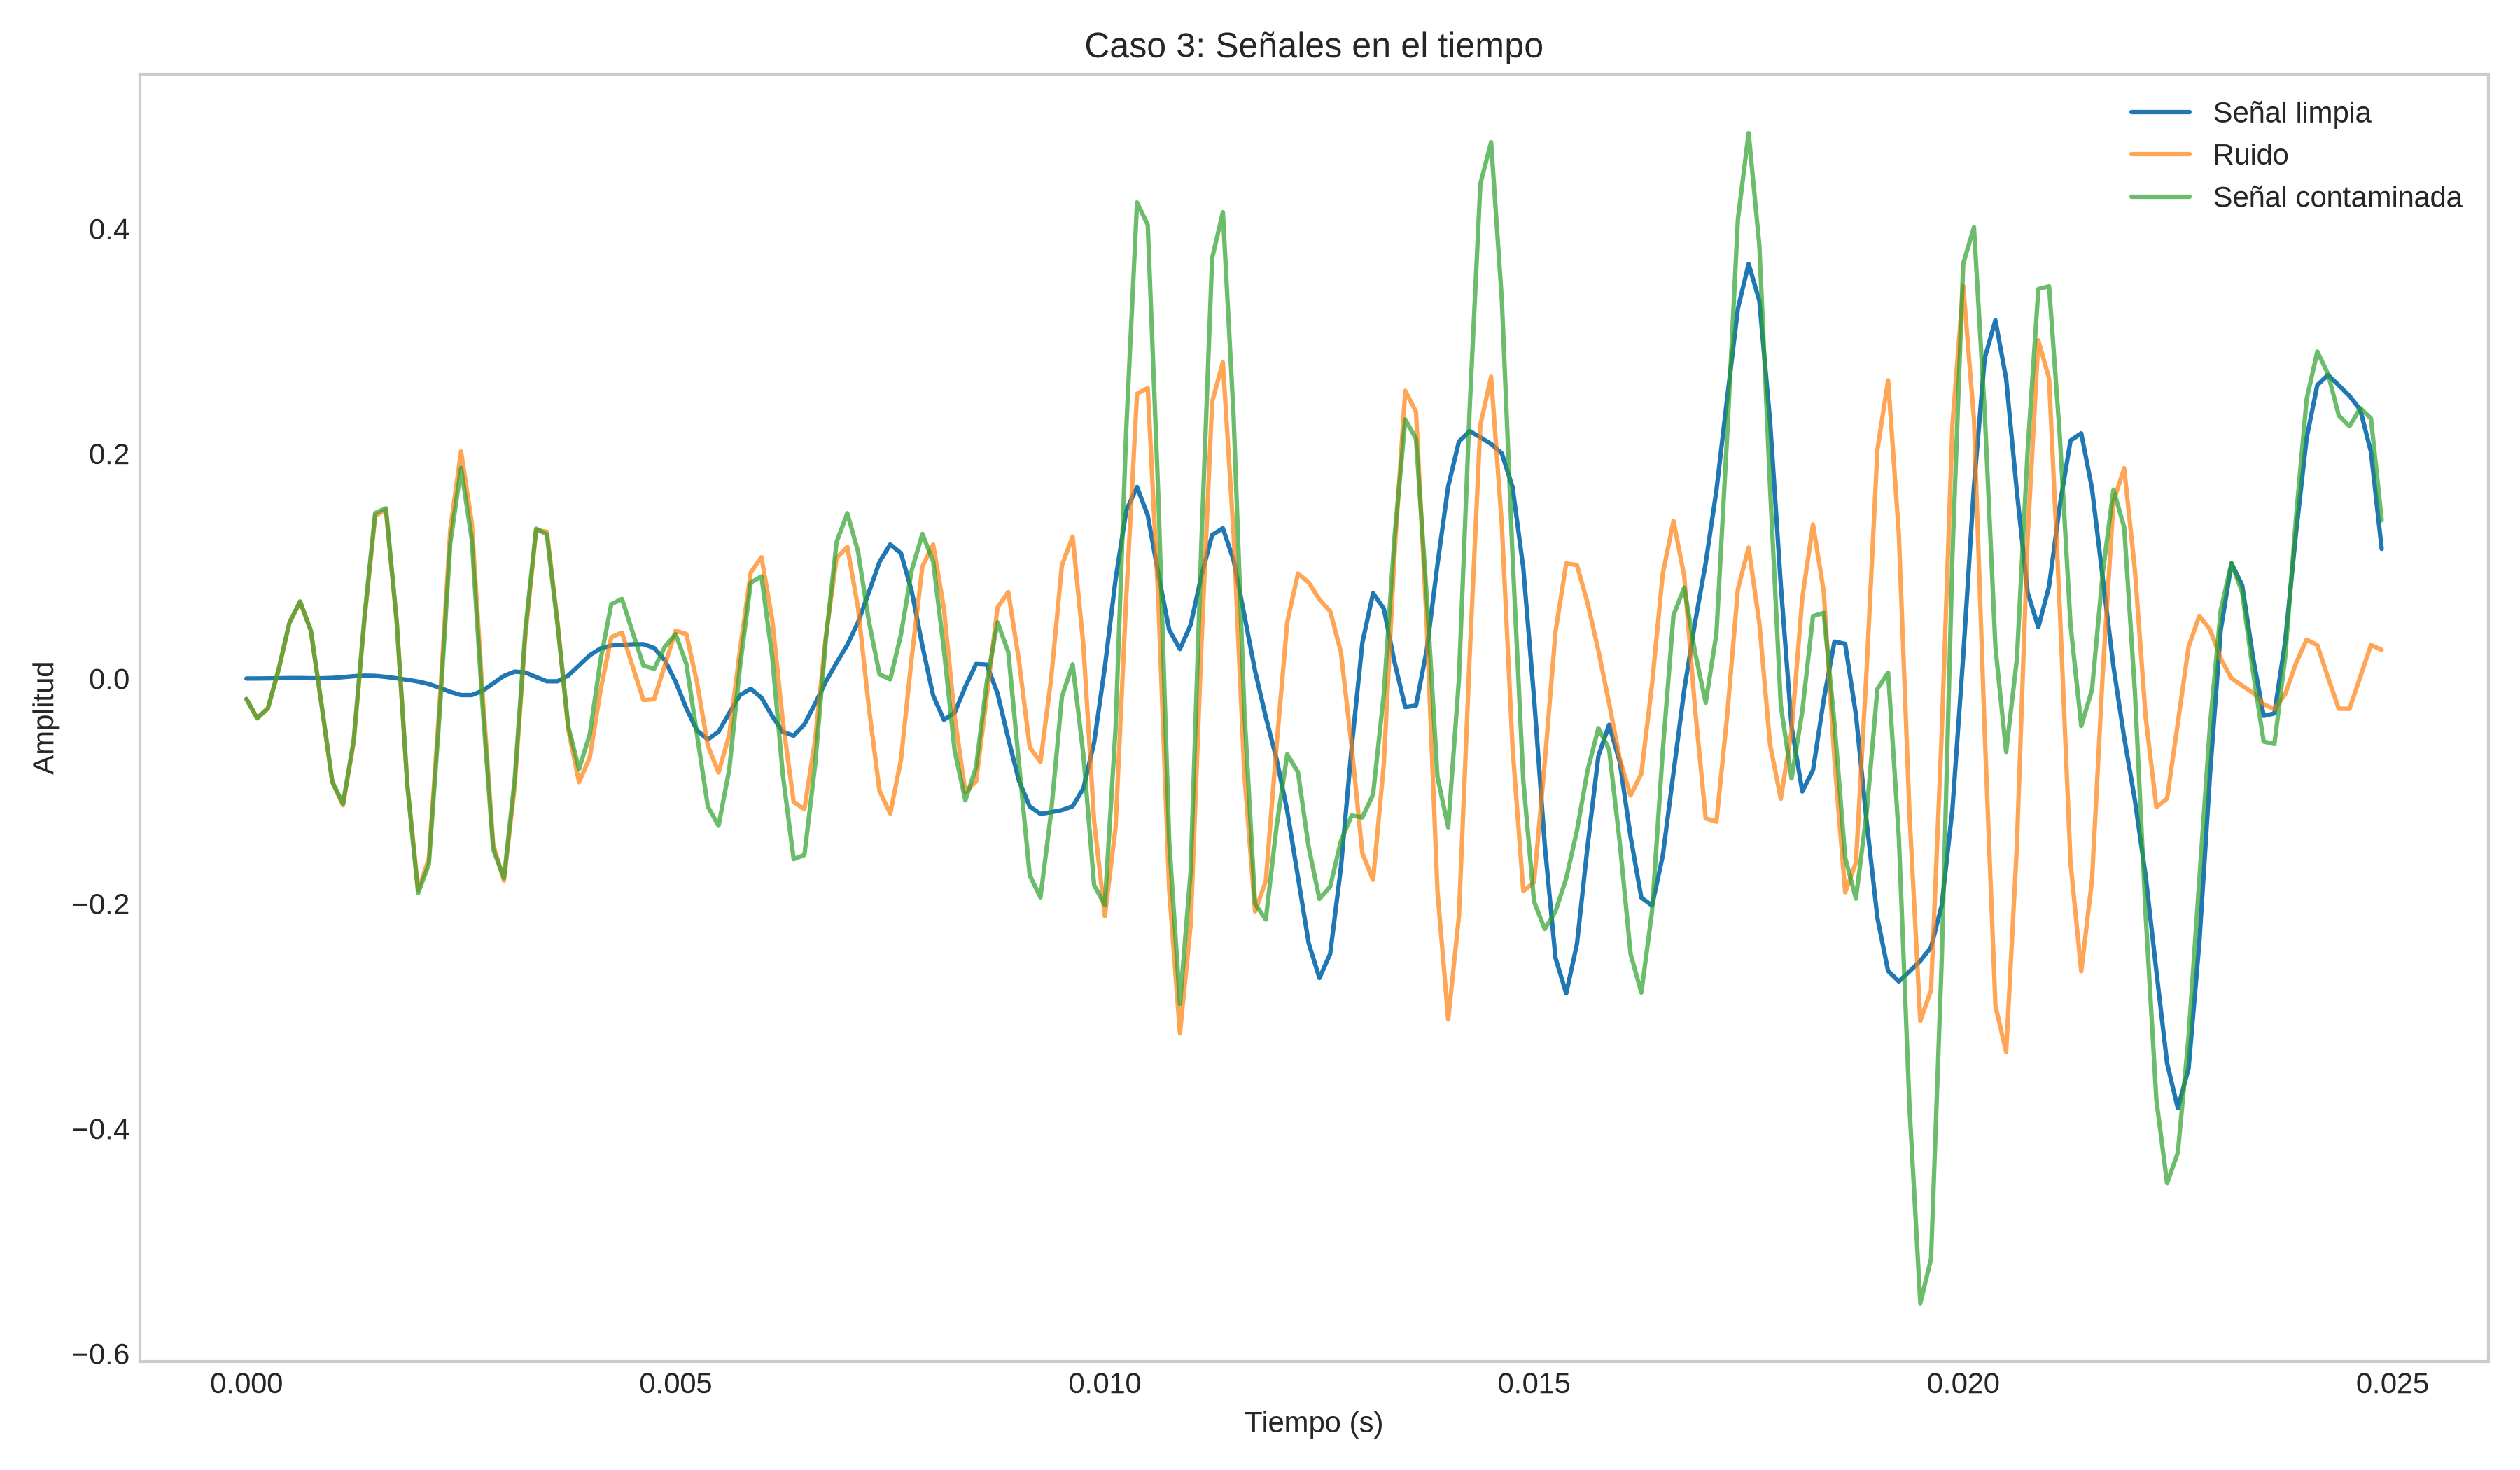
\includegraphics[width=.97\linewidth,height=.38\textheight,keepaspectratio]{generacion_3_temporal.png}\par
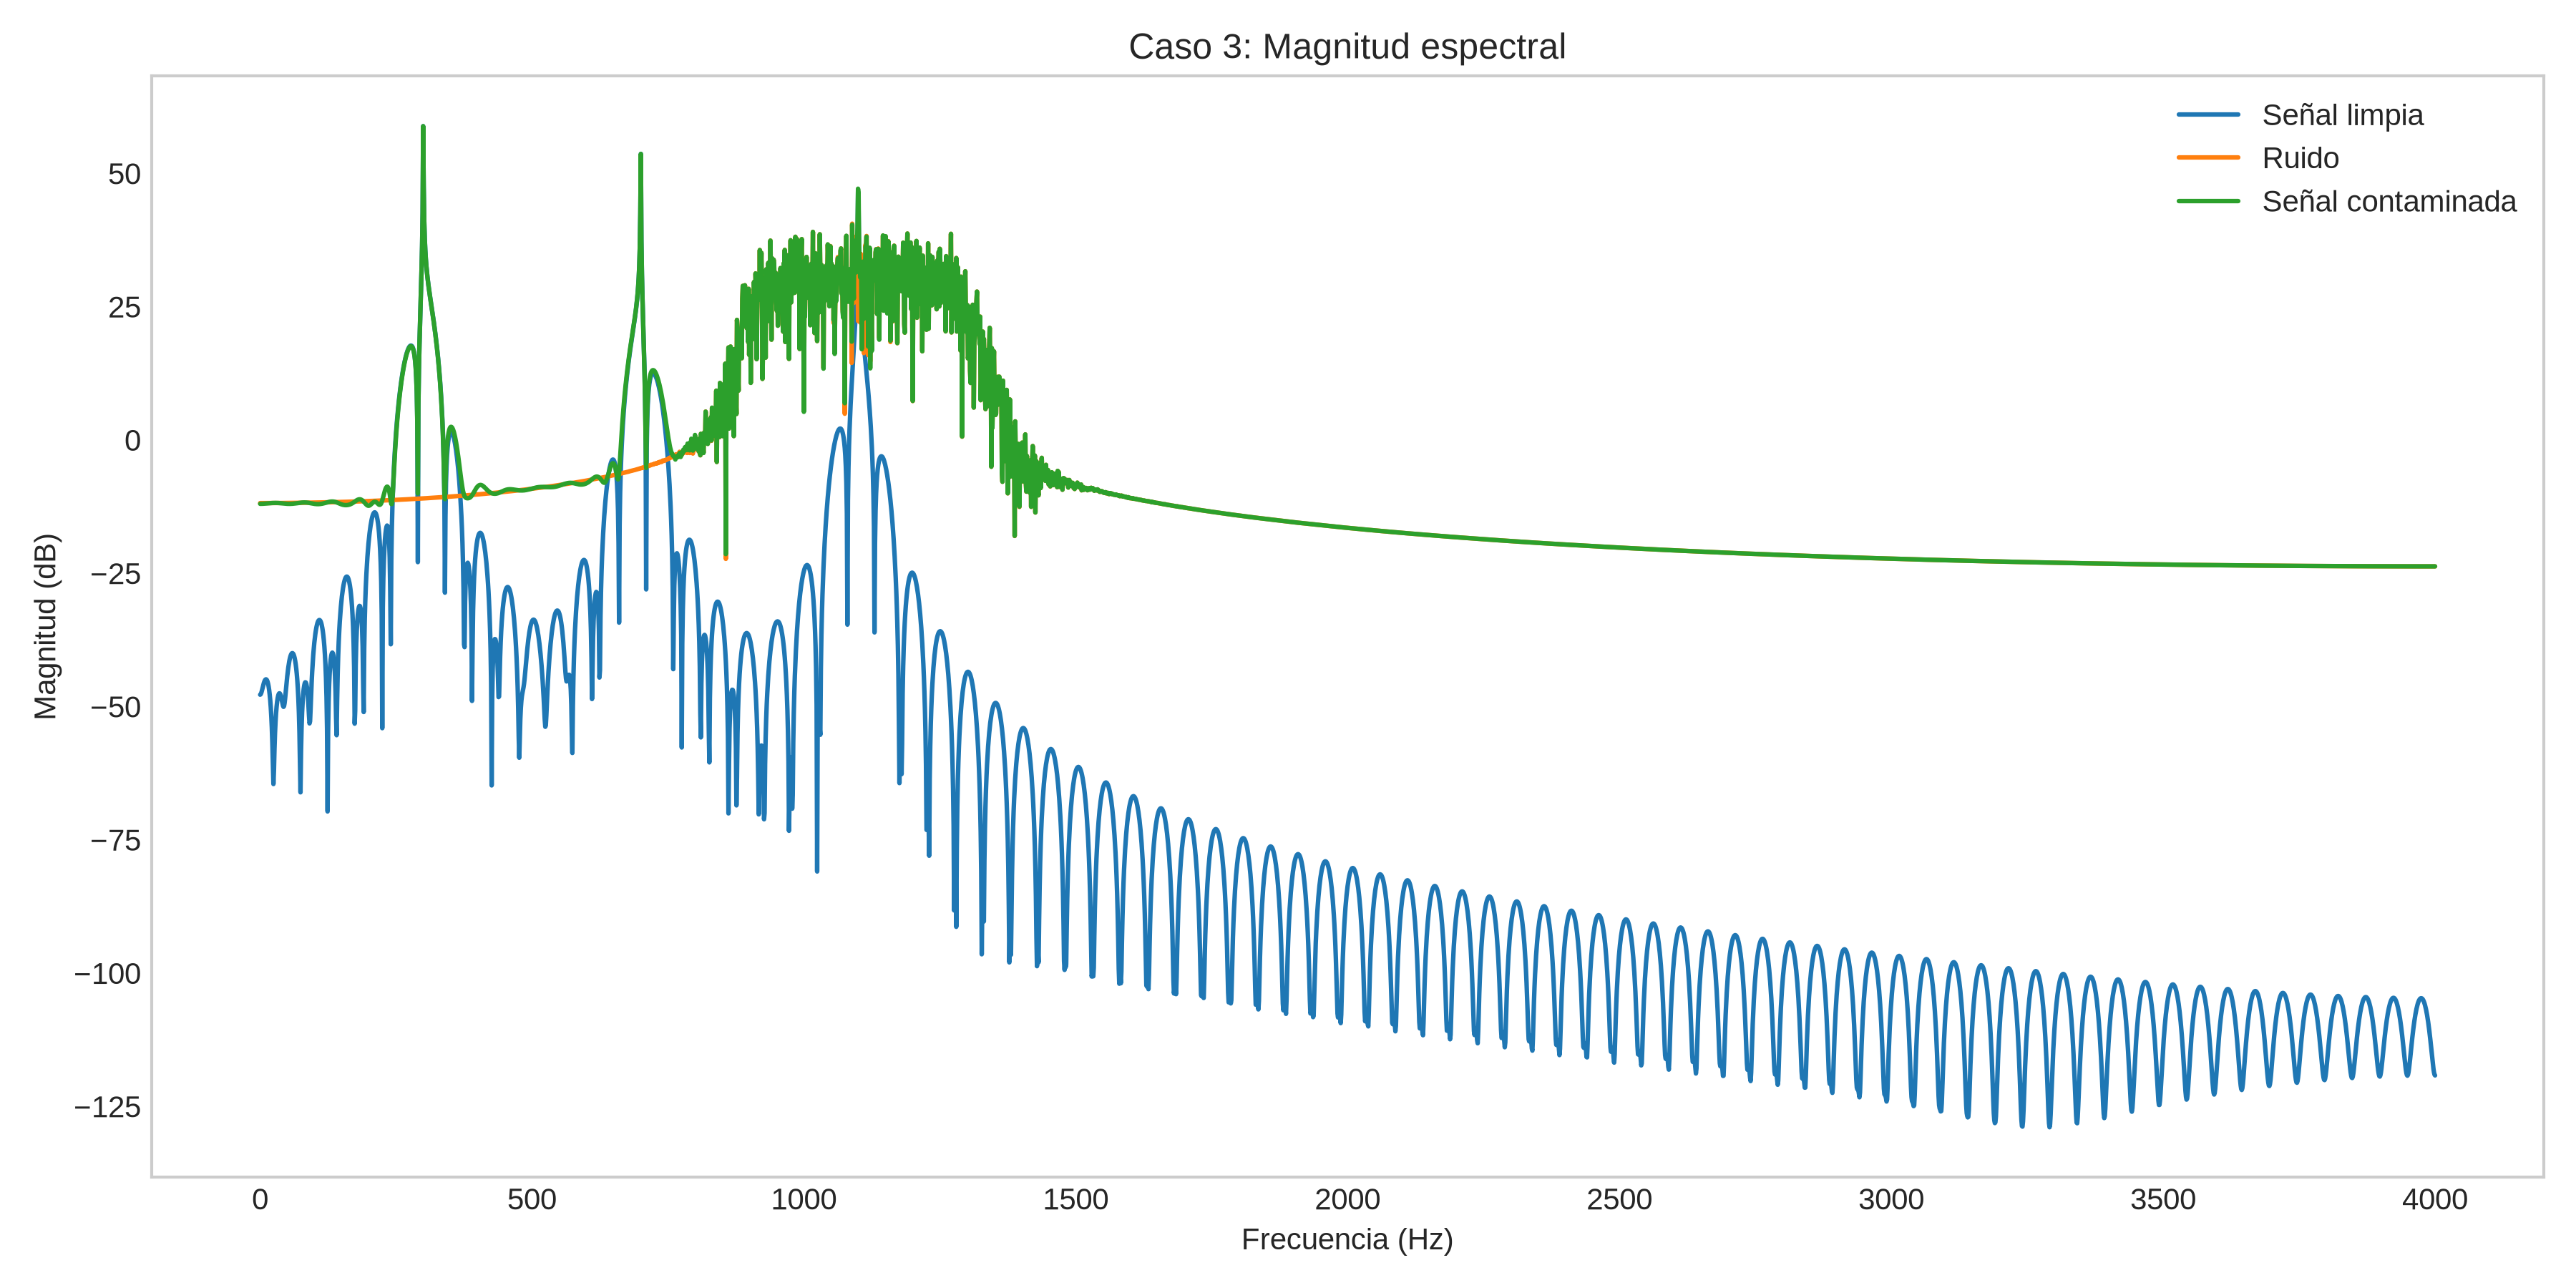
\includegraphics[width=.97\linewidth,height=.38\textheight,keepaspectratio]{generacion_3_magnitud.png}
\caption{Caso 3: Señales temporales y magnitud espectral. Resultados originales de 2.2.}\end{figure}
\begin{figure}[p]\centering
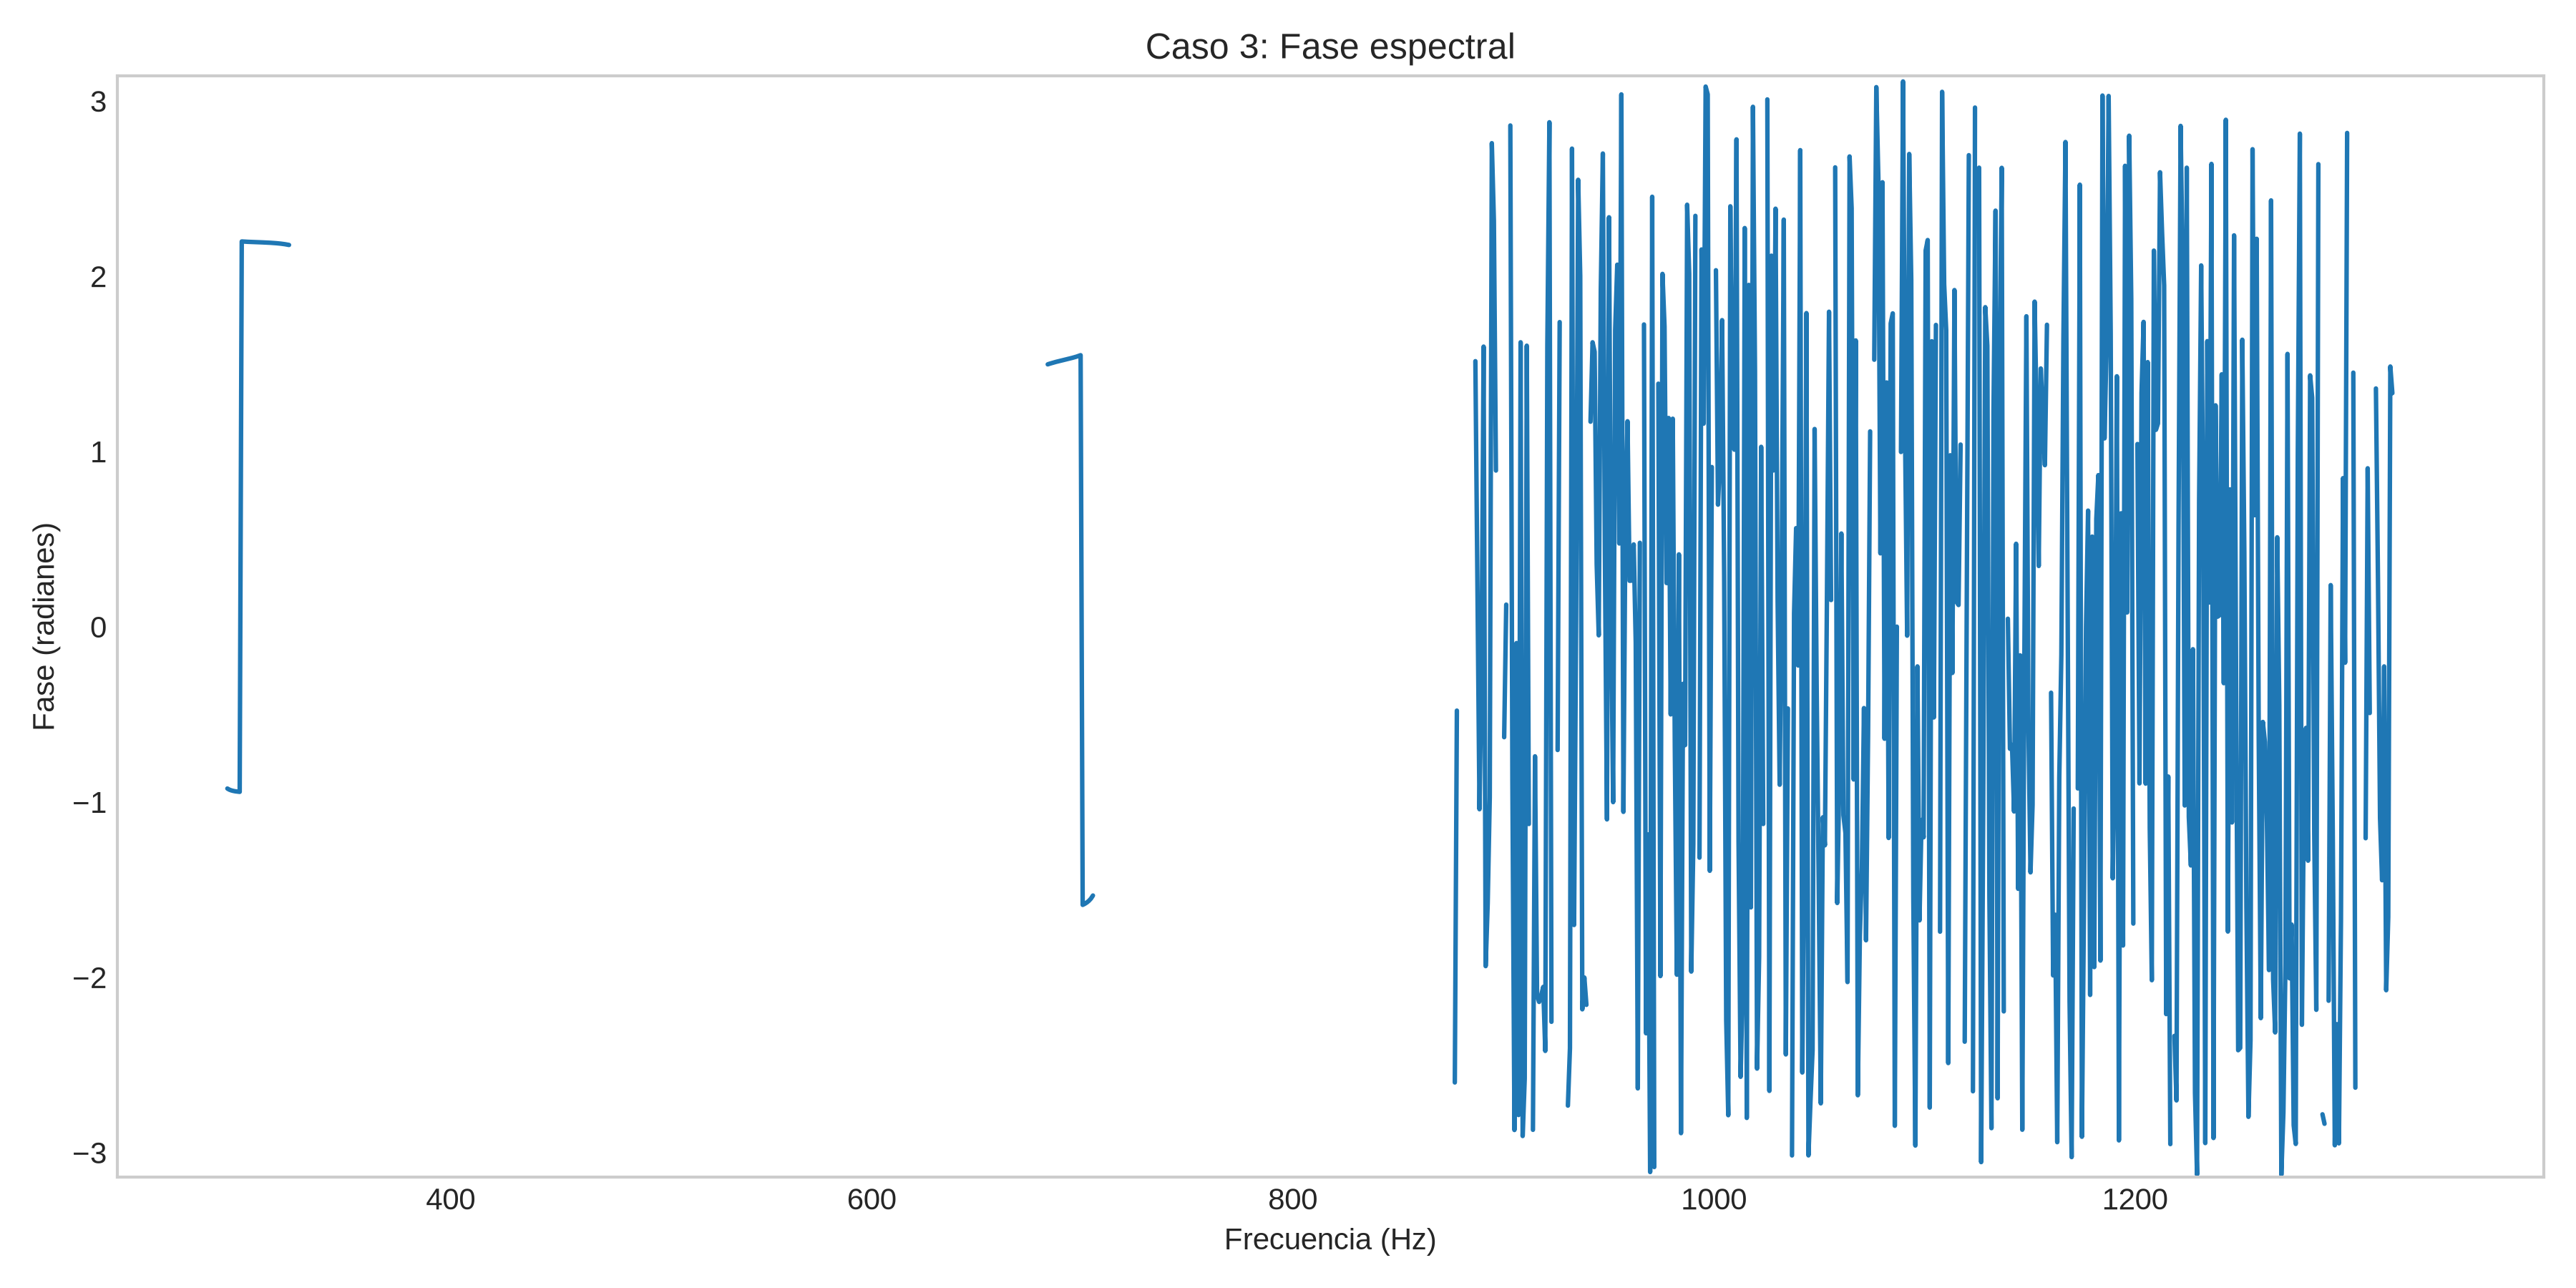
\includegraphics[width=.97\linewidth,height=.38\textheight,keepaspectratio]{generacion_3_fase.png}\par
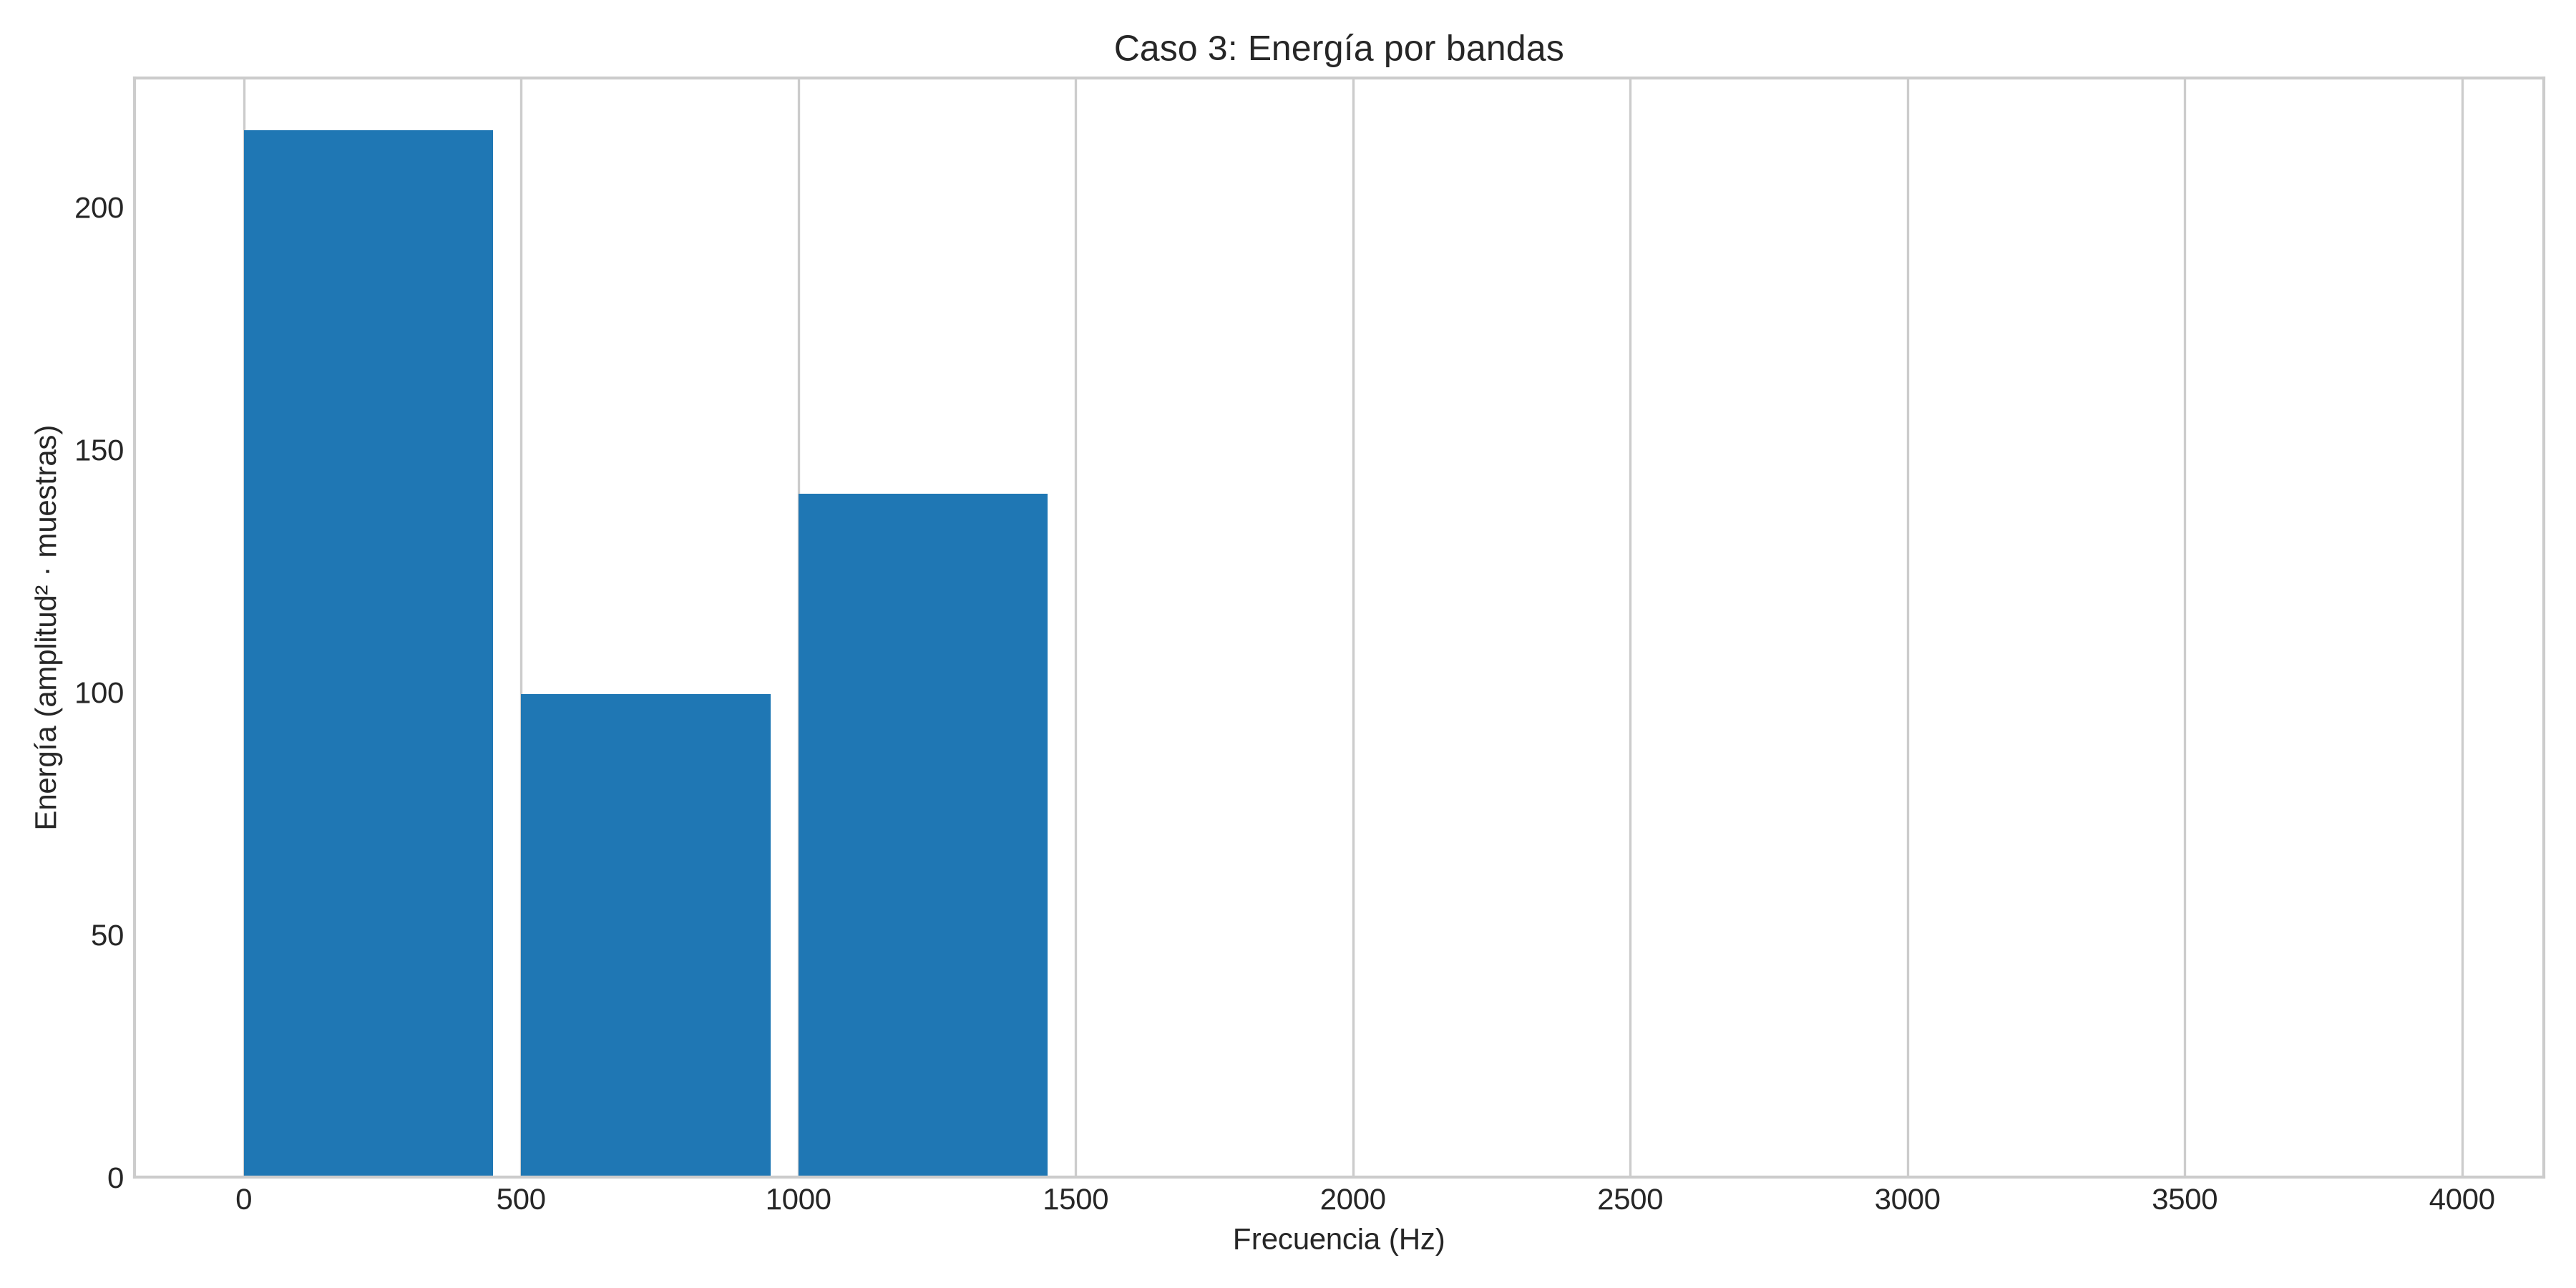
\includegraphics[width=.97\linewidth,height=.38\textheight,keepaspectratio]{generacion_3_energia.png}
\caption{Caso 3: Fase espectral y energía por bandas. Resultados originales de 2.2.}\end{figure}
\clearpage
\subsection{Identificación y límites de recuperación}
El caso 1 tiene un pico detectado a 2150.39 Hz. En el caso 2, la energía entre bandas es casi uniforme, con coeficiente de variación de 3.64\%. En el caso 3, la banda detectada es 870.12--1327.15 Hz; difiere de 900--1300 Hz por la captura finita y la fuga. Estos rasgos ayudan a distinguir ruido tonal, blanco y de banda.

La mezcla no permite separar por completo señal y ruido cuando comparten frecuencias. Rechazar 900--1300 Hz también elimina el tono útil de 1100 Hz. Proteger tonos estables ayuda en estos casos, pero falta probar voz y transitorios.

\section{Filtro temporal FIR (2.3)}
\subsection{Especificaciones y elección}
Se diseña un pasa bajas para el caso 1: paso hasta 1200 Hz, rechazo desde 1800 Hz, pérdida máxima permitida de 1 dB y atenuación mínima de 40 dB. \ruta{firwin} usa corte de 1500 Hz. Kaiser añade 5 dB de margen y se ajusta a 37 coeficientes, de orden 36.

Se comparó con un Butterworth de orden 11: pérdida máxima 0.999 dB, rechazo mínimo 43.489 dB y radio máximo de polos 0.887110. Se eligió FIR por fase lineal, retardo constante y ausencia de realimentación. Su rizado fue 0.062763 dB, pérdida máxima 0.040820 dB y rechazo mínimo 46.106635 dB. A 2150 Hz, la ganancia fue $-64.959$ dB.

\subsection{Ecuación, transferencia, polos y estabilidad}
\begin{equation}
y[n]=\sum_{k=0}^{36}b[k]x[n-k],\qquad
H(z)=\sum_{k=0}^{36}b[k]z^{-k}=\frac{\sum_{k=0}^{36}b[k]z^{36-k}}{z^{36}}.
\end{equation}
Como $b[k]=b[36-k]$, los 19 valores del apéndice definen los 37 coeficientes. $H(z)$ tiene 36 polos en el origen y 36 ceros. Su región de convergencia causal (ROC), $|z|>0$, incluye el círculo unitario. La respuesta al impulso es finita y la suma de sus valores absolutos también lo es, por lo que el filtro es estable\cite{oppenheim,proakis}.
\begin{figure}[H]\centering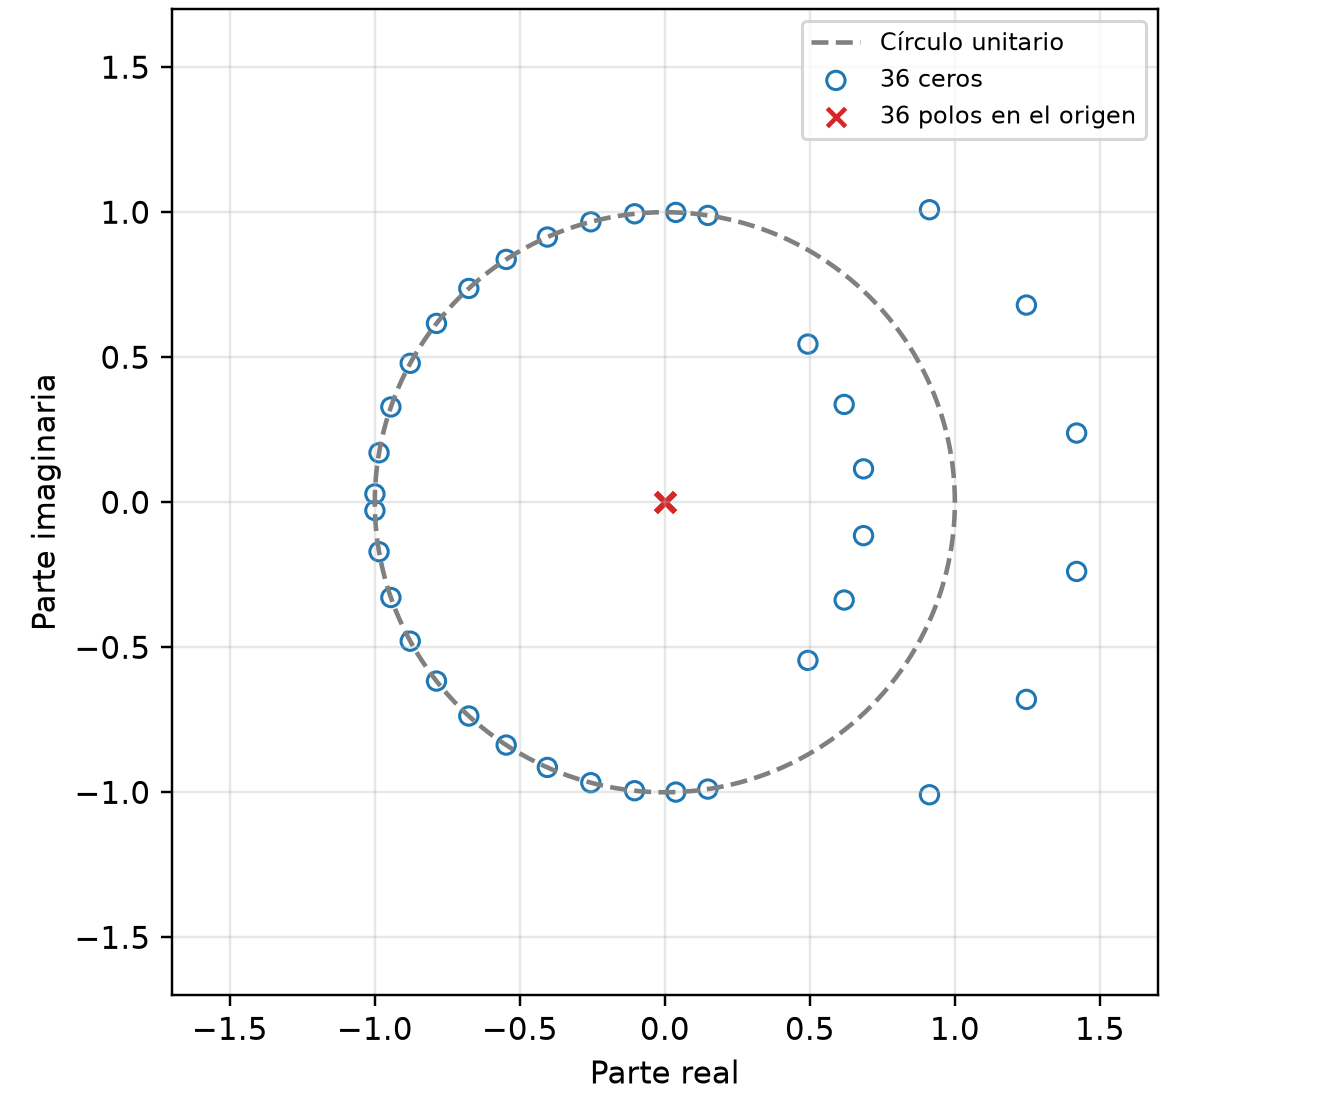
\includegraphics[width=.65\linewidth]{fir_polos_ceros.png}\caption{Polos y ceros del FIR definitivo. Los 36 polos coincidentes se representan con una cruz en el origen.}\end{figure}
\figura{fir_respuesta.png}{Respuesta del FIR definitivo. Magnitud en toda la banda; fase y retardo en banda de paso. El retardo es 18 muestras, equivalente a 2.25 ms.}{fig:fir}

\subsection{Implementación y validación}
La ecuación de diferencias se programa sin una función de filtrado de biblioteca. Frente a \ruta{scipy.signal.lfilter}, los errores máximos de los casos 1--3 fueron $2.776\times10^{-16}$, $3.331\times10^{-16}$ y $3.331\times10^{-16}$, menores que $10^{-12}$. El procesamiento por bloques conserva el estado y reproduce la salida completa; reiniciarlo introduciría transitorios. La comparación de calidad está en 2.5.

\subsection{Cuantización, saturación y memoria}
En \ruta{float32}, el error máximo de coeficiente fue $1.088\times10^{-8}$ y el rechazo mínimo 46.106615 dB. En Q15, punto fijo con paso $2^{-15}=3.052\times10^{-5}$, fueron $1.489\times10^{-5}$ y 45.995639 dB. Ambos cumplen las especificaciones; se propone \ruta{float32}.

Como $\sum_k|b[k]|=1.702778$, se cumple $|y[n]|\leq1.702778\max|x[n]|$. Una entrada en $[-1,1)$ puede exceder ese rango a la salida. Se propone escalar por 0.587276 y contar saturaciones.

La cota del acumulador Q15, 1828323328, cabe en \ruta{int32} (máximo 2147483647); al volver a Q15 se debe controlar la escala. Los 37 coeficientes y 36 estados ocupan 584 B en doble precisión, 292 B en precisión simple o 146 B en Q15. Los datos de control de PC y ESP-DSP se incluyen en 2.5.

\section{Reducción espectral FFT/IFFT (2.4)}
\subsection{Cadena de procesamiento}
El filtro usa $N=1024$ y avanza $H=512$ muestras por bloque, con solape del 50\%. Se aplica raíz de Hann periódica antes de la FFT y después de la IFFT:
\begin{equation}
w[n]=\sqrt{\frac{1-\cos(2\pi n/N)}2},\qquad
w^2[n]+w^2[n+H]=1\quad (0\leq n<H).
\end{equation}
Se resta la media, se rellenan los extremos con ceros y se procesan 17 bloques. Cada bloque pasa por ventana, FFT real, ajuste de ganancias, IFFT y ventana de salida. Se suman las partes superpuestas, se quita el relleno y se restaura la media.

Con ganancias uno, el error de reconstrucción fue menor que $4\times10^{-16}$. Con FFT completa, la parte imaginaria fue menor que $3\times10^{-16}$.

El \emph{piso de ruido} estima la magnitud del ruido por frecuencia. Desde la mezcla se toma la mediana por bin entre bloques y luego una mediana local de 31 bins. Al usar toda la captura, la versión evaluada funciona fuera de línea. Su Hann periódica difiere de la Hann simétrica de 2.1.

\subsection{Reglas adaptativas y selección}
\ruta{picos} detecta máximos locales mayores que seis veces el piso, fuera de 0--1200 Hz. Aplica ganancia $10^{-60/20}=0.001$ al máximo y seis bins por lado. Detecta la frecuencia desde la mezcla, sin recibir 2150 Hz. Con la interferencia movida a 2350 Hz y los mismos parámetros, logró unos 59.33 dB de atenuación alrededor del nuevo tono.

Para los casos de ruido blanco y de banda se usa \ruta{resta}. La ganancia de cada bin $k$ en el bloque $m$ es
\begin{equation}
G_m[k]=\operatorname{clip}\left(1-\frac{3P[k]}{|X_m[k]|},\,0.05,\,1\right).
\end{equation}
$P[k]$ es el piso y $X_m[k]$ el espectro. $\operatorname{clip}$ limita la ganancia a 0.05--1; se evita dividir por magnitudes nulas. Se protegen picos en 0--1200 Hz que superan $2.5$ veces el piso y cuya desviación estándar entre bloques, dividida por su media, es menor que 0.55. Se protege también un bin por lado.

En el caso 3 se detectaron 296.875, 703.125 y 1101.5625 Hz sin usar la referencia limpia. Se elige \ruta{picos} para el caso 1 y \ruta{resta} para 2 y 3 según el ruido configurado. No se ha probado selección automática para señales desconocidas.

\ruta{top_k}, que conserva los 12 bins más intensos, obtuvo 0.03, 17.75 y 7.93 dB de SNR en los casos 1--3 sobre 8192 muestras. \ruta{picos} casi no mejora 2 y 3 porque el ruido ocupa muchas frecuencias. \ruta{resta} deja el caso 1 en 0.14 dB: el tono intenso parece una componente estable y no se reduce bien mediante el piso estimado.

\subsection{Compromiso entre ruido y distorsión}
Se probó el caso 2 sin protección tonal, variando $\alpha$ en $G=\operatorname{clip}(1-\alpha P/|X|,0.05,1)$ sobre las 8192 muestras:
\begin{table}[H]\centering\caption{Prueba con protección tonal desactivada. Atenuación medida fuera de $\pm20$ Hz de los tonos.}
\begin{tabular}{rrrr}\toprule $\alpha$ & Atenuación (dB) & SNR (dB) & Ganancia 1100 Hz (dB)\\\midrule
2&20.62&16.94&$-2.71$\\3&25.85&14.74&$-4.28$\\8&25.98&7.64&$-15.58$\\\bottomrule
\end{tabular}\end{table}
Subir $\alpha$ de 2 a 8 mejora la atenuación fuera de los tonos, pero reduce el tono de 1100 Hz y empeora la SNR. Esta prueba usa parámetros e intervalo distintos de la comparación principal y se presenta aparte.

\section{Comparación y propuesta para ESP32 (2.5)}
\subsection{Cómo se comparan los filtros}
Se usan $K=8192-18=8174$ muestras: índices 0--8173 de referencia, entrada y salida espectral, y 18--8191 de salida FIR. Así se compensa su retardo y se compara el mismo tramo limpio, sin retirar otros extremos. El recorte explica la pequeña diferencia respecto a las SNR objetivo de 0, 5 y 3 dB sobre 8192 muestras.
\begin{align}
\mathrm{MSE}&=\frac1K\sum_{n=0}^{K-1}(s[n]-y[n])^2,\\
\mathrm{SNR}&=10\log_{10}\frac{\sum_n s^2[n]}{\sum_n(s[n]-y[n])^2},\\
\Delta\mathrm{SNR}&=\mathrm{SNR}_{\mathrm{salida}}-\mathrm{SNR}_{\mathrm{entrada}}.
\end{align}
$s[n]$ es la referencia y $y[n]$ la señal evaluada. MSE mide el error medio al cuadrado; SNR compara energía útil y error; $\Delta$SNR mide la mejora. Sin compensar el retardo, el FIR del caso 1 da $-4.998$ dB porque se comparan distintos instantes. Por eso se corrige antes de evaluar calidad.

Para medir energía útil se filtran por separado $s$ y $r$. En el espectral se reutilizan las ganancias aprendidas desde $x$, sin reestimarlas. Se obtienen $y_s$ (aporte útil) y $y_r$ (ruido residual), cuya suma coincide con $y$ dentro de $10^{-12}$. Requiere conocer ambas fuentes y no permite separar mezclas desconocidas en uso normal. Se definen
\begin{equation}
C_u=100\frac{E(y_s)}{E(s)},\qquad A_r=10\log_{10}\frac{E(r)}{E(y_r)},\qquad E(v)=\sum_n v^2[n].
\end{equation}
$C_u$ mide conservación útil y $A_r$ atenuación del ruido. $100E(y)/E(s)$ incluye ruido y términos cruzados: no equivale a $C_u$. Conservar energía tampoco garantiza conservar exactamente la forma de la señal.

$A_B$ se calcula con periodograma unilateral y Hann periódica, duplicando bins interiores para incluir frecuencias negativas. Se evalúan 2130--2170 Hz en el caso 1 y 900--1300 Hz en el 3; para blanco, sin banda dominante, se usa $A_r$. La ganancia útil por tono se ajusta con seno, coseno y DC sobre $y_s$.

\begin{table}[H]\centering\small\caption{Calidad en el mismo intervalo: salidas con el retardo compensado, $K=8174$.}\begin{tabular}{llrrr}\toprule
Caso & Método & MSE & SNR (dB) & $\Delta$SNR (dB)\\\midrule
1 & Entrada & 5.622400e-02 & 0.010 & 0.000\\
1 & FIR & 3.628906e-07 & 51.911 & 51.901\\
1 & FFT/IFFT & 3.422115e-05 & 32.166 & 32.156\\
2 & Entrada & 1.099230e-02 & 5.009 & 0.000\\
2 & FIR & 3.887311e-03 & 9.524 & 4.514\\
2 & FFT/IFFT & 2.888661e-04 & 20.813 & 15.804\\
3 & Entrada & 1.838450e-02 & 3.010 & 0.000\\
3 & FIR & 1.812801e-02 & 3.071 & 0.061\\
3 & FFT/IFFT & 1.252343e-03 & 14.677 & 11.667\\
\bottomrule\end{tabular}
\label{tab:calidad}\end{table}
\begin{table}[H]\centering\small\caption{Energía útil conservada, energía total de salida y atenuación del ruido. $A_B$ no aplica al caso blanco.}\begin{tabular}{llrrrr}\toprule
Caso & Método & $C_u$ (\%) & $E_y/E_s$ (\%) & $A_r$ (dB) & $A_B$ (dB)\\\midrule
1 & Entrada & 100.000 & 199.779 & 0.000 & 0.000\\
1 & FIR & 99.643 & 99.643 & 55.556 & 64.971\\
1 & FFT/IFFT & 100.000 & 100.061 & 32.156 & 59.259\\
2 & Entrada & 100.000 & 132.155 & 0.000 & --\\
2 & FIR & 99.643 & 111.400 & 4.514 & --\\
2 & FFT/IFFT & 99.016 & 100.170 & 17.222 & --\\
3 & Entrada & 100.000 & 151.730 & 0.000 & 0.000\\
3 & FIR & 99.643 & 150.677 & 0.061 & 0.053\\
3 & FFT/IFFT & 99.764 & 104.936 & 11.766 & 11.282\\
\bottomrule\end{tabular}
\end{table}
\begin{table}[H]\centering\small\caption{Ganancia de cada tono útil usando las ganancias calculadas desde la mezcla.}\begin{tabular}{llrrr}\toprule
Caso & Método & 300 Hz (dB) & 700 Hz (dB) & 1100 Hz (dB)\\\midrule
1 & Entrada & 0.0000 & 0.0000 & 0.0000\\
1 & FIR & -0.0170 & -0.0174 & 0.0070\\
1 & FFT/IFFT & 0.0000 & 0.0000 & 0.0000\\
2 & Entrada & 0.0000 & 0.0000 & 0.0000\\
2 & FIR & -0.0170 & -0.0174 & 0.0070\\
2 & FFT/IFFT & -0.0268 & -0.0407 & -0.0795\\
3 & Entrada & 0.0000 & 0.0000 & 0.0000\\
3 & FIR & -0.0170 & -0.0174 & 0.0070\\
3 & FFT/IFFT & -0.0023 & -0.0022 & -0.0827\\
\bottomrule\end{tabular}
\end{table}

\subsection{Resultados y elección por caso}
En el caso 1, el FIR alcanza 51.911 dB frente a 32.166 dB del espectral, conserva 99.643\% de energía útil y su MSE es 94.30 veces menor. El pasa bajas rechaza la interferencia separada de los tonos y requiere poco estado. El espectral atenúa el ruido y conserva casi toda la energía útil, pero deja más error.

Las primeras y últimas 512 muestras concentran 98.983\% de la energía del error espectral del caso 1, aunque ocupan 12.528\% del intervalo. Esto sugiere un efecto de los extremos y las ventanas, sin demostrar la causa. Se mantienen en la comparación.

En el caso 2, el espectral alcanza 20.813 dB frente a 9.524 dB del FIR, conserva 99.016\% de energía útil y mejora la SNR en 15.804 dB. El FIR deja pasar el ruido blanco dentro de su banda; el espectral puede reducirlo en más frecuencias.

En el caso 3, el espectral logra 14.677 dB frente a 3.071 dB del FIR y conserva 99.764\% de energía útil. El FIR casi no mejora porque el ruido coincide con su banda de paso y el tono de 1100 Hz. El espectral protege el tono, pero deja ruido residual.

Se elige FIR para el tono interferente separado y FFT/IFFT para el ruido blanco y de banda probados. La decisión depende del ruido y la señal útil.

\figura{resumen_calidad.png}{Resumen de SNR y MSE con el protocolo común.}{fig:calidad}
\figura{energia_y_tonos.png}{Energía y ganancia de los tonos útiles al aplicar las ganancias obtenidas desde la mezcla.}{fig:energia}
\figura{caso_1_comparacion.png}{Caso 1: comparación temporal, espectral y del error. La vista temporal es una selección de 100--120 ms; las métricas usan todo el intervalo común.}{fig:caso1}
\figura{caso_2_comparacion.png}{Caso 2: ruido distribuido y mejora del método espectral.}{fig:caso2}
\figura{caso_3_comparacion.png}{Caso 3: superposición con la banda útil y ruido residual después del filtrado.}{fig:caso3}
Las gráficas usan 8174 muestras, Hann periódica y no retiran DC. El límite de $-160$ dB es solo visual y no modifica métricas. El error incluye ruido residual y distorsión.

\subsection{Tiempo y memoria medidos en PC}
Se hicieron tres ejecuciones previas y 30 repeticiones por caso, alternando métodos. \ruta{perf_counter_ns} mide solo filtrado, sin carga, diseño, métricas ni exportación. El tiempo equivalente por 1024 muestras es la mediana de captura dividida entre ocho, no una latencia de tiempo real.
\begin{table}[H]\centering\footnotesize\caption{Mediciones en PC: tiempo equivalente por 1024 muestras, percentil 95 de la captura y memoria persistente y pico. El equivalente se obtiene de la mediana de captura.}\begin{tabular}{llrrrr}\toprule
Caso & Método & Eq. 1024 (ms) & P95 captura (ms) & Persist. (B) & Pico trazado (B)\\\midrule
1 & Entrada & 0.0000 & 0.000 & 0 & 0\\
1 & FIR & 6.1635 & 72.844 & 592 & 133329\\
1 & FFT/IFFT & 0.1228 & 2.262 & 0 & 989751\\
2 & Entrada & 0.0000 & 0.000 & 0 & 0\\
2 & FIR & 5.2720 & 45.915 & 592 & 133329\\
2 & FFT/IFFT & 0.2504 & 2.259 & 0 & 1067580\\
3 & Entrada & 0.0000 & 0.000 & 0 & 0\\
3 & FIR & 5.8214 & 47.989 & 592 & 133329\\
3 & FFT/IFFT & 0.1613 & 1.563 & 0 & 1067487\\
\bottomrule\end{tabular}
\end{table}
Se usó un Intel Core i5-12450H. El FIR manual de Python y las operaciones de NumPy tienen costos distintos de implementación; sus tiempos no predicen el rendimiento en ESP32.

\ruta{tracemalloc} mide el pico adicional y puede omitir reservas nativas. La entrada ocupa 65536 B y se cuenta aparte. El FIR conserva 592 B: 37 coeficientes $b$, uno $a$ y 36 estados en doble precisión. El espectral no conserva estado entre capturas, pero reserva RAM durante la llamada. Persistencia y pico pueden compartir datos y no se suman.
\figura{recursos_pc.png}{Tiempo y memoria del prototipo en PC. Las cifras no son mediciones del sistema físico.}{fig:pc}
\subsection{Parámetros y procesamiento en tiempo real para ESP32}
Se proponen tres ESP32 clásicos, $f_s=8000$ Hz, $N=1024$, avance $H=512$ y \ruta{float32}. Hay 7.8125 Hz entre bins y llega un lote cada 64 ms. Procesar el FIR en lotes de 512 en vez de 1024 no cambia la salida si conserva sus coeficientes y estado.

La estimación en tiempo real debe usar solo muestras recibidas. Para DC se propone $d[n]=d[n-1]+\beta(x[n]-d[n-1])$, con $\beta=1-e^{-1/(f_s\tau)}$ y $\tau=1$ s. Se inicia con la primera muestra y se guarda DC por índice para restaurarlo en la salida correspondiente.

El piso usaría el bloque actual y siete anteriores, con mediana por bin y mediana local de 31 bins. Se mantienen inicialmente $\alpha=3$, ganancia mínima 0.05 y los umbrales de detección. Hasta reunir ocho bloques se usa ganancia uno; el relleno no entra al estimador. Los 576 ms abarcan el historial, no el retardo de reproducción.

La meta es procesar, incluido diagnóstico, en $\leq48$ ms de los 64 ms entre lotes. El FIR requiere 18944 multiplicaciones y acumulaciones por lote, 296000/s. Una FFT radix 2 de 1024 puntos tiene 5120 mariposas (operaciones de combinación), 10240 para FFT e IFFT. Estos conteos no son ciclos de CPU ni prueban cumplimiento del plazo.

En placa se comprobarán identidad con ganancias uno, continuidad y error menor que $10^{-5}$ en precisión simple. Se propone perder como máximo 1 dB de SNR respecto a PC en el mismo intervalo. Son metas, todavía no resultados en ESP32.

Se verificarán antialias, conversores y reloj. En el ejemplo I2S con dos posiciones de 32 bits, 512 muestras ocupan 4096 B, más que el límite DMA de 4092 B. Se usarían dos descriptores de 256 muestras y 2048 B\cite{espidf}. El formato depende del ADC elegido.

\subsection{Bibliotecas: licencia, precisión y restricciones}
ESP-DSP 1.8.2 tiene licencia Apache 2.0 y requiere ESP-IDF $\geq4.2$ según su configuración\cite{espdsp}. Se revisó su código, sin compilar firmware. \ruta{dsps_fft2r_fc32} usa partes reales e imaginarias intercaladas en precisión simple, con optimización ESP32 y máximo 1024. \ruta{dsps_bit_rev2r_fc32} ordena la FFT. La inversa es
\begin{equation}\operatorname{IFFT}(X)=\frac{\operatorname{conj}(\operatorname{FFT}(\operatorname{conj}(X)))}N.\end{equation}
Cada par conjugado recibe la misma ganancia; DC y Nyquist se modifican una vez. El arreglo complejo ocupa 8192 B y las tablas 4096 B de rotaciones y 1984 B de ordenamiento. Se inicializan una vez, sin creación/liberación simultánea desde varias tareas.

El FIR necesita 41 posiciones de estado, 37 coeficientes y una estructura de control estimada de 40 B en plataforma de 32 bits: 352 B. El orden de coeficientes debe probarse con un FIR no simétrico, pues invertir el actual ocultaría el error. ESP32-S3 exige revisar sus restricciones propias.

KISS FFT 131.1.0 usa licencia BSD de tres cláusulas\cite{kiss}. Su formato por defecto es \ruta{float}; admite doble precisión y Q15/Q31. La FFT real exige longitud par; entrada y salida en el mismo arreglo pueden requerir memoria adicional; la IFFT flotante necesita normalización. Se elige ESP-DSP por su optimización ESP32, pendiente de medir en placa.

\subsection{Arquitectura de tres nodos}
\figura{arquitectura_nodos.png}{Funciones de los tres ESP32 y sus enlaces UART. Los tiempos son estimaciones que deben medirse en las placas.}{fig:nodos}
N1 adquiere $x$, asigna índices y calcula un resumen FFT. N2 aplica FIR y reproduce con DAC/PWM y filtro de reconstrucción. N3 aplica FFT/IFFT, reproduce, compara las rutas y muestra métricas.

N1 envía $x$ a N2 y N3, y $s$ a N3 en pruebas con referencia. N2 envía $y_{\mathrm{FIR}}$ a N3. UART0 queda para consola y los otros dos UART para enlaces\cite{uart}, a 3.3 V y tierra común. Los pines dependen de la placa y sus periféricos.

En prueba digital, N1 reproduce $x$ y $s$ con reloj e índices comunes. Una referencia analógica requiere calibrar y sincronizar conversores. Sin referencia, MSE, SNR y energía útil se indican como no disponibles.

N3 estima ganancias desde $x$ y las aplica a $s$ con otra FFT/IFFT y estado propio para medir energía útil. Otra instancia FIR procesa la referencia. La atenuación por ventanas cortas se etiqueta como estimación por bloque, distinta de la medición de 8174 muestras.

\subsection{Formato de paquetes y velocidad de comunicación}
Cada enlace UART envía y recibe a la vez a 921600 baudios, 8N1: ocho bits de datos, uno de inicio y uno de parada. El paquete incluye cabecera de 32 B, datos, CRC de 4 B, COBS y un cero delimitador\cite{cobs,zlib}. COBS evita ceros internos; el CRC comprueba cabecera y datos antes de codificarlos. Se usa CRC-32/ISO-HDLC, polinomio reflejado \ruta{0xEDB88320}, inicio y XOR final \ruta{0xFFFFFFFF}. La prueba \ruta{123456789} da \ruta{0xCBF43926}.

Los campos de la cabecera se envían con el byte menos significativo primero. Sus 32 B se distribuyen así: identificador (2 B); versión, tipo, origen y destino (1 B cada uno); banderas (2 B); sesión y secuencia (4 B cada una); índice de la primera muestra (8 B); cantidad de muestras (2 B); formato y número de canales (1 B cada uno); longitud de datos (4 B).

Un canal contiene 512 muestras finitas y normalizadas en \ruta{float32}: 2048 B. Si se envían $x$ y $s$, se intercalan. Los índices FIR se mantienen como salida causal; el retardo de 18 muestras se compensa solo al calcular calidad.

DIAG (64 B) resume muestreo, bloque, avance, método, estado del estimador, frecuencia/banda, piso, DC, energía, tiempo, contadores, índice y configuración. Control (32 B) permite configurar, iniciar, detener, consultar y confirmar. Los parámetros se preinstalan; los cambios se confirman e indican su primer índice efectivo.

Si $R$ es el tamaño de cabecera, datos y CRC, el tamaño máximo reservado tras COBS es $R+\lfloor R/254\rfloor+2$, incluido el delimitador:
\begin{table}[H]\centering\caption{Tamaños máximos por paquete.}\begin{tabular}{lrrr}\toprule Tipo&Carga (B)&Cabecera+carga+CRC (B)&Enlace (B)\\\midrule Entrada o FIR&2048&2084&2094\\Entrada con referencia&4096&4132&4150\\DIAG&64&100&102\\Control&32&68&70\\\bottomrule\end{tabular}\end{table}
Se envían $f_s/H=15.625$ lotes por segundo. Para $B$ bytes por lote, la tasa mínima en 8N1 es $10Bf_s/H$ baudios:
\begin{table}[H]\centering\small\caption{Tasa requerida por enlace, incluido un DIAG por lote desde N1.}\begin{tabular}{lrrr}\toprule Enlace&B/lote&Mínimo (baudios)&Uso a 921600\\\midrule N1--N2: $x$+DIAG&2196&343125&37.23\%\\N1--N3: $(x,s)$+DIAG&4252&664375&72.09\%\\N2--N3: FIR&2094&327187.5&35.50\%\\\bottomrule\end{tabular}\end{table}
Sin referencia, N1--N3 requiere lo mismo que N1--N2. Diez controles/s por sentido añaden 7000 baudios medios: el enlace más cargado llega a 671375, el 72.85\% de 921600. 115200 es insuficiente. Al ser independientes, las tasas no se suman como un bus compartido.

Se verifican tamaño máximo 4150 B, CRC, sesión, destino, formato e índices. Estos detectan audio perdido o repetido; perder DIAG no implica perder muestras. No se reenvía audio vencido. Una pérdida invalida métricas, se registra y reinicia estados y estimación con transición controlada de salida.

La recepción UART sigue activa durante el filtrado. Los índices alinean muestras, pero no corrigen deriva de relojes: se requiere reloj común o ajustar reproducción según la ocupación de las colas FIFO.

\subsection{Memoria y retardo estimados}
El procesamiento espectral por sí solo requiere unos 65133 B, o 81517 B al incluir sus reservas auxiliares. El cálculo completo por nodo añade la referencia, el FIR, la lectura de paquetes y la memoria de UART, DMA, tareas y colas:
\begin{table}[H]\centering\caption{RAM estimada por nodo. Debe comprobarse con el firmware completo.}\begin{tabular}{lrrrr}\toprule Nodo&Total (B)&Total (KiB)&Meta (KiB)&Margen (B)\\\midrule N1&72868&71.16&96&25436\\N2&46652&45.56&64&18884\\N3&137377&134.16&160&26463\\\bottomrule\end{tabular}\end{table}
N3 guarda referencia y salida FIR en dos FIFO de 2048 muestras, 8192 B cada una. Reserva 40960 B auxiliares; N1 y N2, 32768 B cada uno. La RAM se comprobará con firmware completo; no equivale al pico medido en Python.

Se propone un retardo de reproducción de 256 ms, cuatro avances de 64 ms. El cálculo supone filtrado en hasta 48 ms, entrega a UART en 1 ms por enlace, envío simultáneo desde N1 y como máximo un control extra por avance. La salida espectral estaría lista en 223.897 ms y la FIR alineada en 226.069 ms, antes de 256 ms. Falta medirlo con conversores, colas e interrupciones. El retardo propio del FIR sigue siendo 18 muestras, 2.25 ms.

\section{Conclusiones}
Las pruebas muestran que la elección del filtro depende de cómo se distribuye el ruido respecto a las frecuencias útiles. Para la interferencia tonal separada, el FIR obtuvo 51.911 dB de SNR frente a 32.166 dB del espectral. En cambio, FFT/IFFT dio mejores resultados con ruido blanco y de banda superpuesto, con 20.813 y 14.677 dB. Por tanto, el FIR resulta adecuado cuando puede rechazar el ruido sin afectar la banda útil; el método espectral ofrece mayor mejora en los otros dos casos probados.

Cuando señal y ruido comparten frecuencias, eliminar una banda completa también elimina información útil. La protección de tonos permitió reducir ese daño, pero dejó ruido residual. La prueba sin protección mostró además que aumentar la sustracción puede empeorar la SNR. Por eso la elección debe considerar tanto la reducción del ruido como la distorsión de la señal, en lugar de buscar únicamente la mayor atenuación.

La comparación usó las mismas señales y un intervalo común, compensando las 18 muestras de retardo del FIR. Esto permitió evaluar la calidad sin penalizar un desplazamiento temporal conocido. También se distinguió la energía útil de la energía total de salida, que incluye ruido. Estos criterios permiten interpretar las métricas sin confundir una salida de mayor energía con una mejor recuperación.

La propuesta para tres ESP32 define el procesamiento, la comunicación y la memoria necesaria, pero aún requiere pruebas en placa. Los tiempos medidos en PC no demuestran que se cumplan los plazos del sistema embebido. El siguiente paso será implementar la estimación con muestras presentes y pasadas, y comprobar calidad, uso de RAM y pérdidas de comunicación. Los resultados actuales quedan como referencia para esa validación.

\section{Aportes, archivos de respaldo y uso de IA}
\begin{table}[H]\centering\caption{Distribución conforme al plan inicial.}\begin{tabular}{lp{10cm}}\toprule Responsable&Aporte\\\midrule Integrante 1&Fundamentos, demostraciones FFT y generación/caracterización (2.1--2.2).\\Integrante 2&Diseño FIR/IIR, ecuación de diferencias y validación temporal (2.3).\\Integrante 3&Estimación adaptativa y reconstrucción espectral (2.4).\\Integrante 4&Protocolo común, comparación, bibliotecas, arquitectura e informe (2.5).\\\bottomrule\end{tabular}\end{table}
El código y los resultados están en \ruta{seccion_2_1/} a \ruta{seccion_2_5/}. \ruta{seccion_2_5/src/evaluar_comparacion.py} usa \ruta{revision/paso_2/protocolo.json} y guarda métricas en CSV.

Las figuras se generan desde esos datos con \ruta{seccion_2_5/src/graficar_comparacion.py}.

Las tablas e imágenes del informe se preparan con \ruta{informe/preparar_recursos.py}, sin volver a medir tiempos.

\ruta{revision/} guarda pruebas, cálculos y huellas de archivos. CRC/COBS se verificaron en PC, no en un enlace físico. El notebook y paquete están en \ruta{entrega/tarea1/}; la etiqueta prevista de entrega es \ruta{tarea1_prototipo}.

Se usó IA como apoyo para explicar conceptos sobre filtros y otros temas del trabajo, y para comparar el filtrado temporal con el espectral. También se utilizó para elaborar scripts, generar gráficos y verificar los datos calculados. Al final, ayudó a integrar los aportes de cada integrante y los borradores en un solo documento.

\clearpage
\begin{thebibliography}{10}
\bibitem{tarea} L. Chavarría Zamora. \emph{Tarea 1: Caracterización espectral y prototipado de filtros para reducción de ruido}. CE1110, TEC, segundo semestre de 2026. Enunciado versión 7.
\bibitem{proyecto} L. Chavarría Zamora. \emph{Diseño de un sistema distribuido de reducción adaptativa de ruido en tiempo real}. CE1110, TEC, segundo semestre de 2026. Enunciado del proyecto, versión 7.
\bibitem{oppenheim} A. V. Oppenheim, A. S. Willsky y S. H. Nawab. \emph{Señales y sistemas}, 2.\textsuperscript{a} ed. Ejemplar proporcionado en \ruta{Contexto/}. Fourier y sistemas lineales; secciones 1.6.6 y 3.8--3.9.
\bibitem{proakis} J. G. Proakis y D. G. Manolakis. \emph{Digital Signal Processing}, 4.\textsuperscript{a} ed. Ejemplar proporcionado en \ruta{Contexto/}. DFT, FFT, ventanas y filtrado; sección 5.4.1.
\bibitem{espdsp} Espressif Systems. \emph{ESP-DSP}, versión 1.8.2: licencia, manifiesto, FFT y FIR. \url{https://github.com/espressif/esp-dsp/tree/v1.8.2}. Consulta: 12 de octubre de 2026.
\bibitem{kiss} M. Borgerding y colaboradores. \emph{KISS FFT}, versión 131.1.0: README y licencia. \url{https://github.com/mborgerding/kissfft/tree/131.1.0}. Consulta: 12 de octubre de 2026.
\bibitem{espidf} Espressif Systems. \emph{ESP-IDF: I2S driver, ESP32}. \url{https://docs.espressif.com/projects/esp-idf/en/stable/esp32/api-reference/peripherals/i2s.html}. Consulta: 12 de octubre de 2026.
\bibitem{uart} Espressif Systems. \emph{ESP-IDF: UART driver, ESP32}. \url{https://docs.espressif.com/projects/esp-idf/en/stable/esp32/api-reference/peripherals/uart.html}. Consulta: 12 de octubre de 2026.
\bibitem{cobs} S. Cheshire y M. Baker. \emph{Consistent Overhead Byte Stuffing}. \url{https://www.stuartcheshire.org/papers/COBSforToN.pdf}.
\bibitem{zlib} J. L. Gailly y M. Adler. \emph{zlib manual} y \ruta{crc32.c}, versión 1.3.1. \url{https://zlib.net/manual.html}; \url{https://github.com/madler/zlib/blob/v1.3.1/crc32.c}. Consulta: 12 de octubre de 2026.
\end{thebibliography}
\clearpage
\appendix
\section{Coeficientes del FIR definitivo}
Cada fila define $b[k]=b[36-k]$; el central aparece una sola vez. $a[0]=1$ y no hay realimentación.
\begin{center}\small\begin{tabular}{rrr}\toprule $k$ & $36-k$ & $b[k]=b[36-k]$\\\midrule
0 & 36 & $1.1281118305568869\mathrm{e}-03$\\
1 & 35 & $2.3012855797120866\mathrm{e}-03$\\
2 & 34 & $-2.6611140796740475\mathrm{e}-18$\\
3 & 33 & $-4.6418238294469606\mathrm{e}-03$\\
4 & 32 & $-4.7669952206183322\mathrm{e}-03$\\
5 & 31 & $3.3770127372078889\mathrm{e}-03$\\
6 & 30 & $1.1336913791783341\mathrm{e}-02$\\
7 & 29 & $5.4957536078769128\mathrm{e}-03$\\
8 & 28 & $-1.2734199171669404\mathrm{e}-02$\\
9 & 27 & $-2.0730780518584790\mathrm{e}-02$\\
10 & 26 & $1.0245579273282646\mathrm{e}-17$\\
11 & 25 & $3.2081736006478692\mathrm{e}-02$\\
12 & 24 & $3.0810901887059709\mathrm{e}-02$\\
13 & 23 & $-2.1259777528944767\mathrm{e}-02$\\
14 & 22 & $-7.2924291746006925\mathrm{e}-02$\\
15 & 21 & $-3.8636615819073801\mathrm{e}-02$\\
16 & 20 & $1.0998222858046637\mathrm{e}-01$\\
17 & 19 & $2.9201113153602493\mathrm{e}-01$\\
18 & 18 & $3.7433881655435630\mathrm{e}-01$\\
\bottomrule\end{tabular}
\end{center}
\end{document}
